\chapter*{第六部分:情绪、动机和体内平衡的生物学}
\markboth{总论}{总论}

\begin{figure}[htbp]
	\centering
	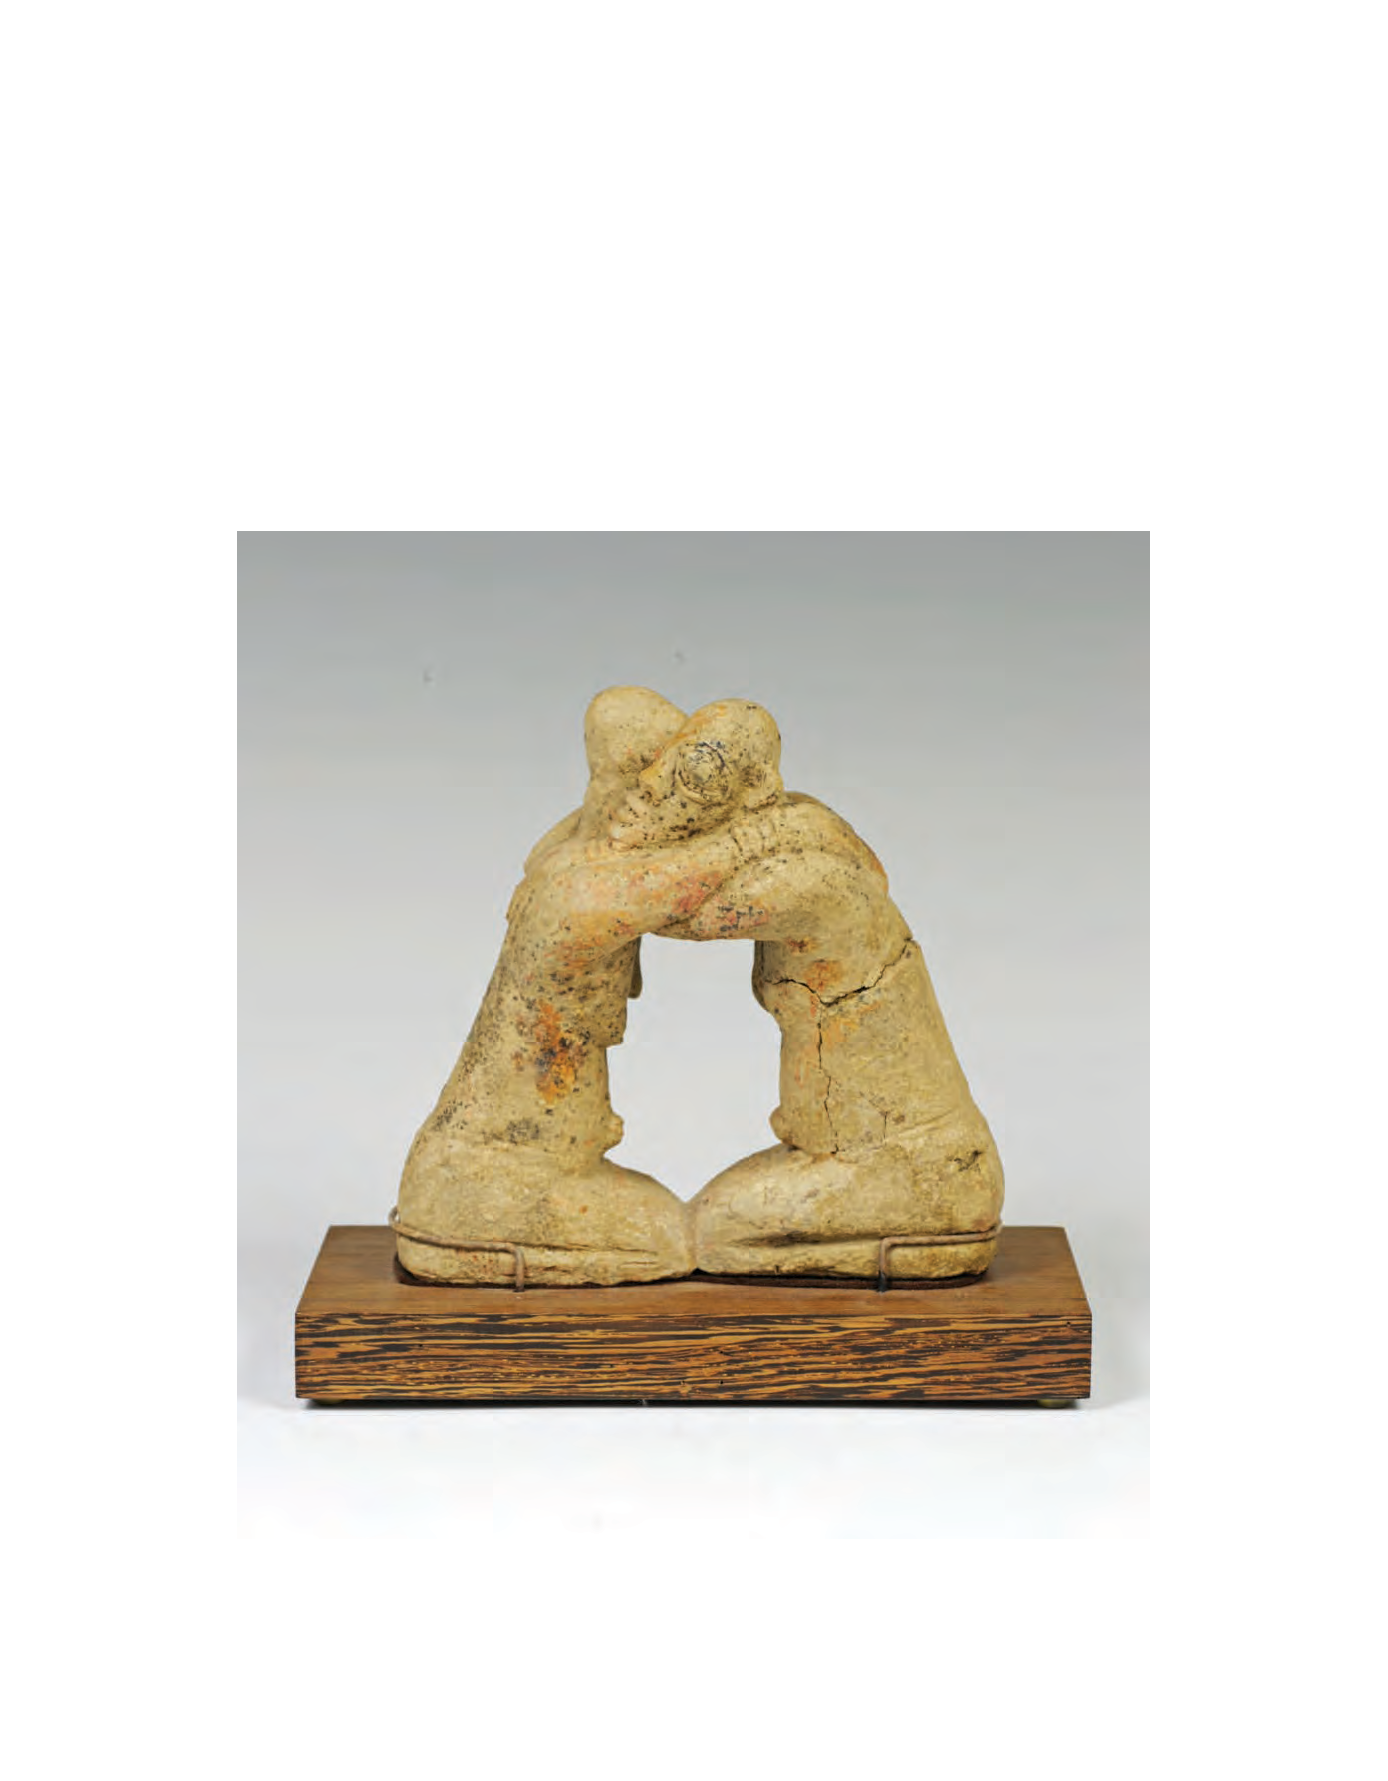
\includegraphics[width=0.95\linewidth]{chap40/fig_40_0}
	\caption{拥抱的夫妇哀悼某人的死亡,也许埋在附近的骨灰盒里。
		(马里,詹尼风格。
		尼日尔河内陆三角洲,公元 13-15 世纪。
		爱荷华大学斯坦利艺术博物馆,斯坦利非洲艺术收藏。)}
	\label{fig:40_0}
\end{figure}


情绪和稳态行为都涉及一个或多个躯体,自主,激素或认知过程的协调。
皮层下大脑区域涉及一系列功能,包括进食,饮酒,心率,呼吸,温度调节,睡眠,性别和面部表情,在这种协调中起着至关重要的作用。
皮层下大脑区域与皮层大脑区域双向连接,为内部状态变量(例如内脏信息)的重新表达提供了一种手段,以影响认知操作,例如主观感受,决策和注意力,认知功能可以调节或消除皮层下大脑区域的神经表征,从而帮助协调反映情绪状态的行为。


我们对这些系统的考虑始于脑干,脑干一方面对清醒和有意识的注意力至关重要,另一方面对睡眠至关重要。
位于脊髓和间脑之间的大脑这个小区域的重要性与其大小不成比例。
脑干的损伤会严重影响运动和感觉过程,因为它包含所有将感觉信息从身体表面传递到大脑皮层的上行通道,以及所有将运动命令传递到脊髓的大脑皮层下行通道。
最后,脑干包含控制呼吸和心跳的神经元,以及产生支配头部和颈部的大部分颅神经的细胞核。


脑干中的六个神经化学调节系统调节感觉,运动和唤醒系统。
连接中脑与边缘系统和皮层的多巴胺能通路特别重要,因为它们参与处理与强化期望有关的刺激和事件,因此有助于动机状态和学习。
人们认为,尼古丁、酒精、阿片类药物和可卡因等成瘾性药物通过选择相同的神经通路产生作用,这些神经通路可以积极增强生存所必需的行为。
其他调节性递质部分通过控制丘脑和皮层之间的信息流来调节睡眠和觉醒。
皮层丘脑回路中的电兴奋异常可导致癫痫发作和癫痫发作。


脑干的头端是下丘脑,它的功能是通过将生理变量保持在有利于重要身体过程的范围内来维持内部环境的稳定性。
神经系统的稳态过程对行为产生了深远的影响,这引起了许多现代生理学创始人的兴趣,包括\textit{克劳德$\cdot$伯纳德}、\textit{沃尔特$\cdot$坎农}和\textit{沃尔特$\cdot$赫斯}。
控制内部环境的神经元集中在下丘脑,这是间脑的一小部分,占大脑总体积的不到1\%。
下丘脑在脑干和边缘系统中具有紧密相连的结构,通过控制内分泌系统和自主神经系统,直接作用于内部环境,以实现目标导向的行为。
它通过与大脑高级区域的连接间接调节情绪和动机状态。
除了影响动机行为外,下丘脑以及下方的脑干和上方的大脑皮层还保持着一种普遍的觉醒状态,从兴奋和警惕到嗜睡和昏迷。


情绪的神经生物学研究依赖于实验,这些实验根据特定的测量来定义情绪,从人类情绪的主观报告,接近或防御行为,到自主反应等生理反应。
\textit{查尔斯$\cdot$达尔文}在他的开创性著作《人类和动物的情绪表达》中观察到,许多情绪在物种间是保守的,这清楚地表明了通过使用动物模型来探索神经机制来研究情绪的相关性。
因此,在实验框架中,情绪状态被认为是大脑的中枢状态,可以引起物种间协调的行为,生理和认知反应。


近年来,关于情绪的许多研究都集中在杏仁核上,杏仁核可以通过与皮层,下丘脑和脑干的连接来协调不同的反应。
人类杏仁核的损伤会损害恐惧的学习和表达,以及其他人的恐惧识别,这是由于人们对传达恐惧的面部特征的注意力分配减少。
从成瘾到焦虑再到社交缺陷,各种精神疾病的症状都可能涉及杏仁核功能障碍。
然而,杏仁核只是一组较大大脑区域的一个组成部分,其中包括下丘脑,脑干和皮层区域的一部分,这些区域也负责协调情绪反应。
特别是,内侧和腹侧前额叶皮层和杏仁核紧密相连。
这些结构内部和之间的动态处理可能会超越协调的情绪行为,包括灭绝,情绪状态的认知调节,社交和情绪领域之间的相互作用,以及杏仁核表征对决策和主观感受的影响。




\chapter{脑干} \label{chap:chap40}

在原始脊椎动物(爬行动物、两栖动物和鱼类)中,前脑只是大脑的一小部分,主要用于嗅觉处理以及自主神经和内分泌功能与生存所必需的基本行为的整合。
这些基本行为包括进食、饮水、有性繁殖、睡眠和应急反应。
尽管我们习惯于认为前脑协调大多数人类行为,但许多复杂的反应,例如进食——咀嚼、舔舐和吞咽的协调——实际上是由相对简单的、刻板的运动反应组成的,这些反应由前脑中的神经元集合控制。


通过观察出生时没有前脑的婴儿(水脑畸形),可以清楚地看出这种组织模式在人类行为中的重要性。
脑积水婴儿很难与正常婴儿区分开来。 他们会哭、会笑、会吃奶,还会活动他们的眼睛、脸、胳膊和腿。
正如这些悲惨的案例所表明的,脑干几乎可以组织新生儿的所有行为。


在本章中,我们描述了脑干的功能解剖结构,尤其是颅神经,以及组织面部和头部简单行为的局部回路神经元的集合。
最后,我们考虑了脑干中核团的调节功能,这些调节功能可调节感觉、运动和唤醒系统的敏感性。


脑干是脊髓的延髓,其运动和感觉成分在结构上与脊髓相似。
但是控制脑神经的脑干部分比控制脊神经的脊髓相应部分复杂得多,因为脑神经介导更复杂的行为。
脑干的核心,即网状结构,与脊髓的中间灰质同源,但也更复杂。
与脊髓一样,网状结构包含局部回路中间神经元的集合,这些中间神经元产生运动和自主模式并协调反射和简单行为。
此外,脑干包含调节觉醒、清醒-睡眠周期、呼吸和其他重要功能的谷氨酸能和氨基丁酸能回路,以及可优化神经系统功能的单胺能调节神经元。



\section{颅神经与脊神经同源}

由于脊神经只到达第一颈椎,颅神经为头部提供躯体和内脏、感觉和运动神经支配。
两条颅神经,舌咽神经和迷走神经,也提供颈部、胸部和除骨盆外的大部分腹部器官的内脏感觉和运动神经支配。
此外,一些颅神经与特殊功能相关,例如视觉或听觉,这些功能超出了脊髓的感觉和运动计划。


颅神经评估是神经系统检查的重要部分,因为功能异常可以查明脑干中受损的部位。
因此,重要的是要了解颅神经的起源、它们在颅内的走行以及它们从颅骨中出来的位置。


颅神经传统上按头尾顺序编号为 I 到 XII。
I 和 II 颅神经进入前脑底部。
其他脑神经起源于脑干的特征位置(图~\ref{fig:40_1})。
除了一个从脑干的腹面出口外,其余的都出口(图~\ref{fig:40_2})。
滑车 (IV) 神经是个例外,它从下丘后面的背表面离开中脑,并缠绕在脑干的外侧表面以连接与眼球运动有关的其他颅神经。
具有感觉功能的颅神经(V、VII、VIII、IX 和 X)具有相关的感觉神经节,其功能与背根神经节对脊神经的作用非常相似。
这些神经节位于进入颅骨时沿着单个神经的通路。


\begin{figure}[htbp]
	\centering
	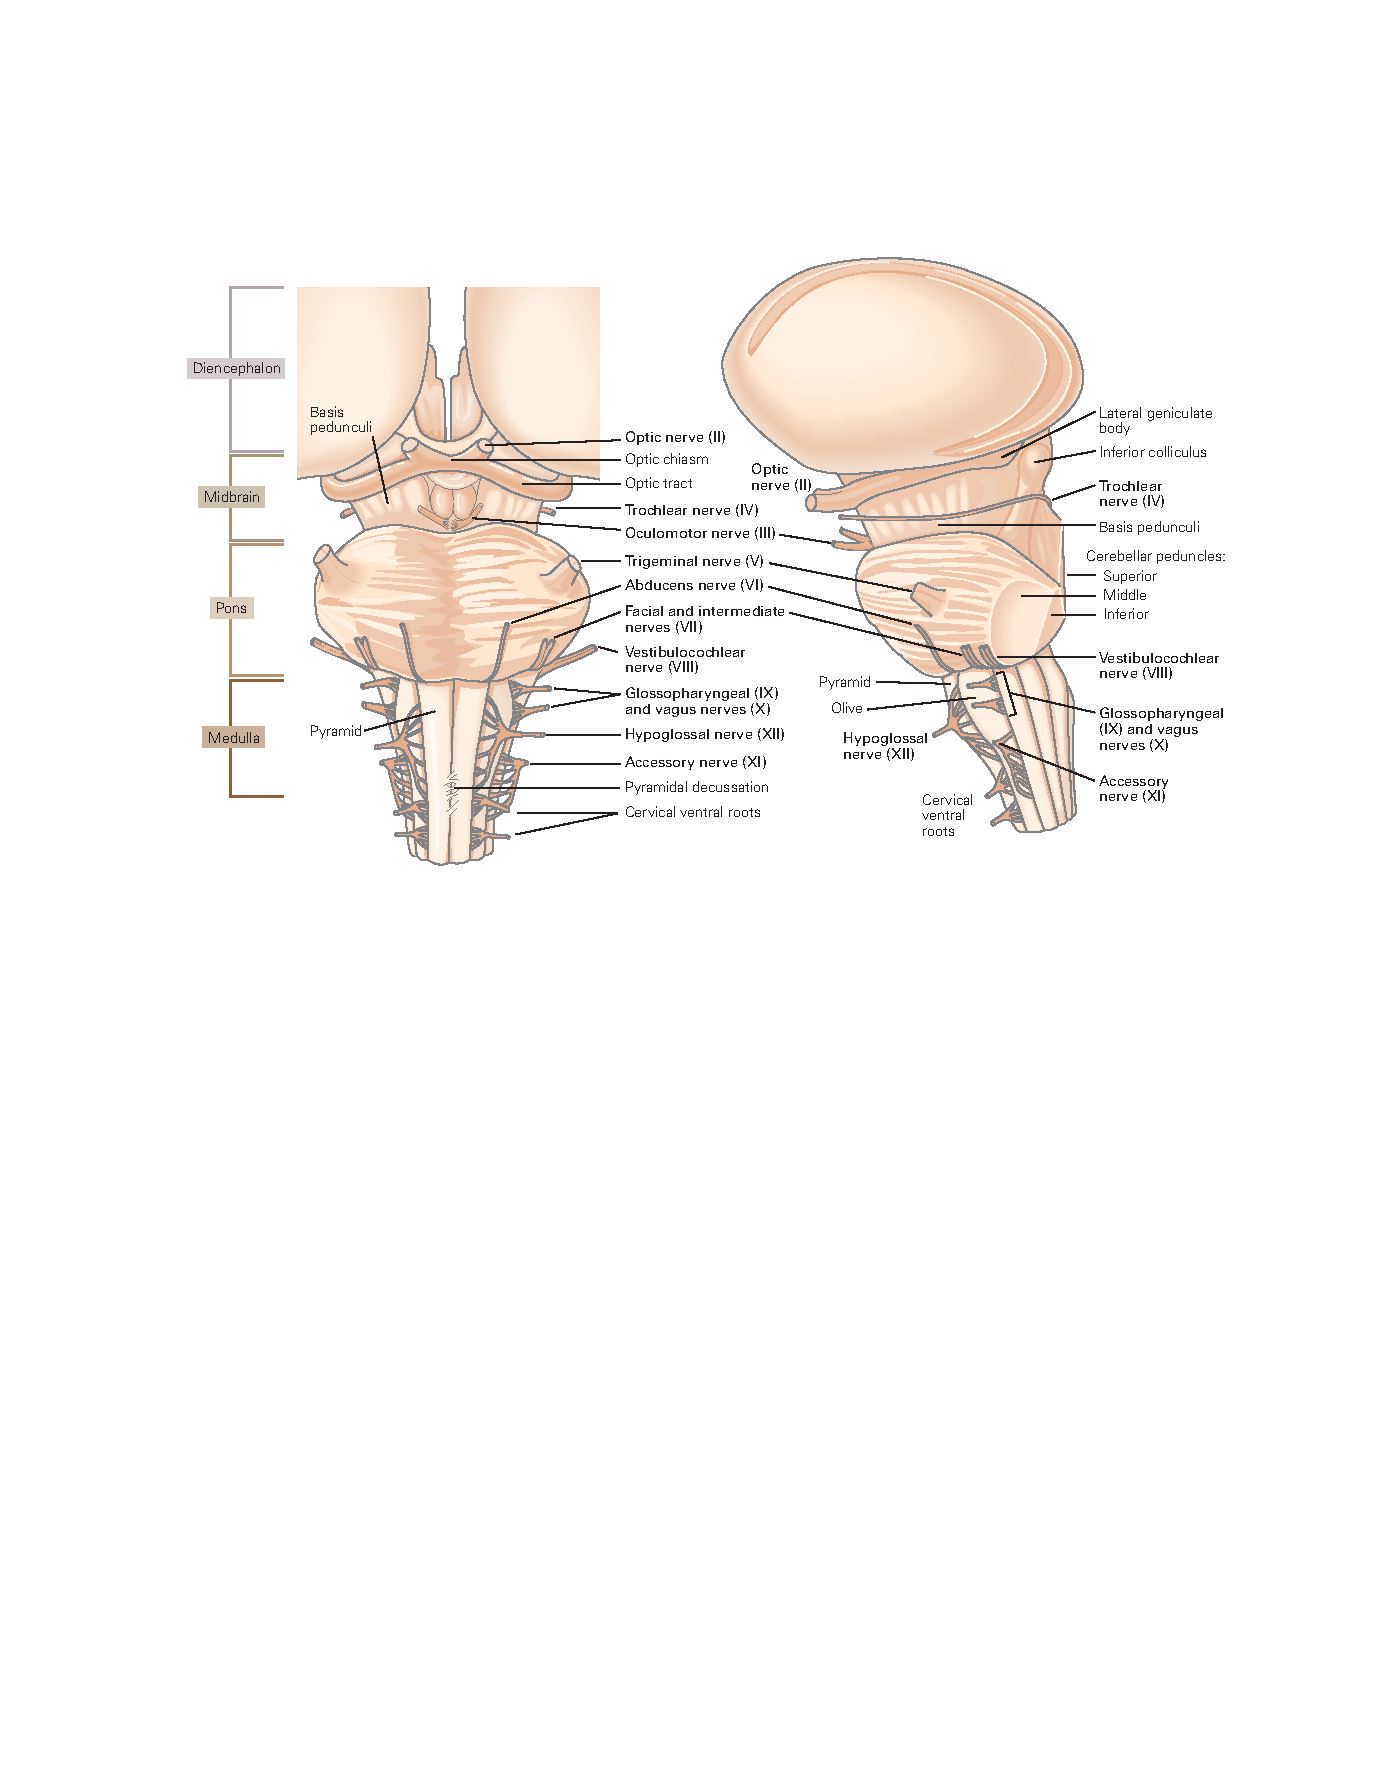
\includegraphics[width=1.0\linewidth]{chap40/fig_40_1}
	\caption{脑干中颅神经的起源(腹侧和侧视图)。
		嗅觉 (I) 神经未显示,因为它终止于前脑的嗅球。 除了一个脑神经外,所有的脑神经都从大脑的腹侧表面发出; 滑车 (IV) 神经起源于中脑的背表面。}
	\label{fig:40_1}
\end{figure}


\begin{figure}[htbp]
	\centering
	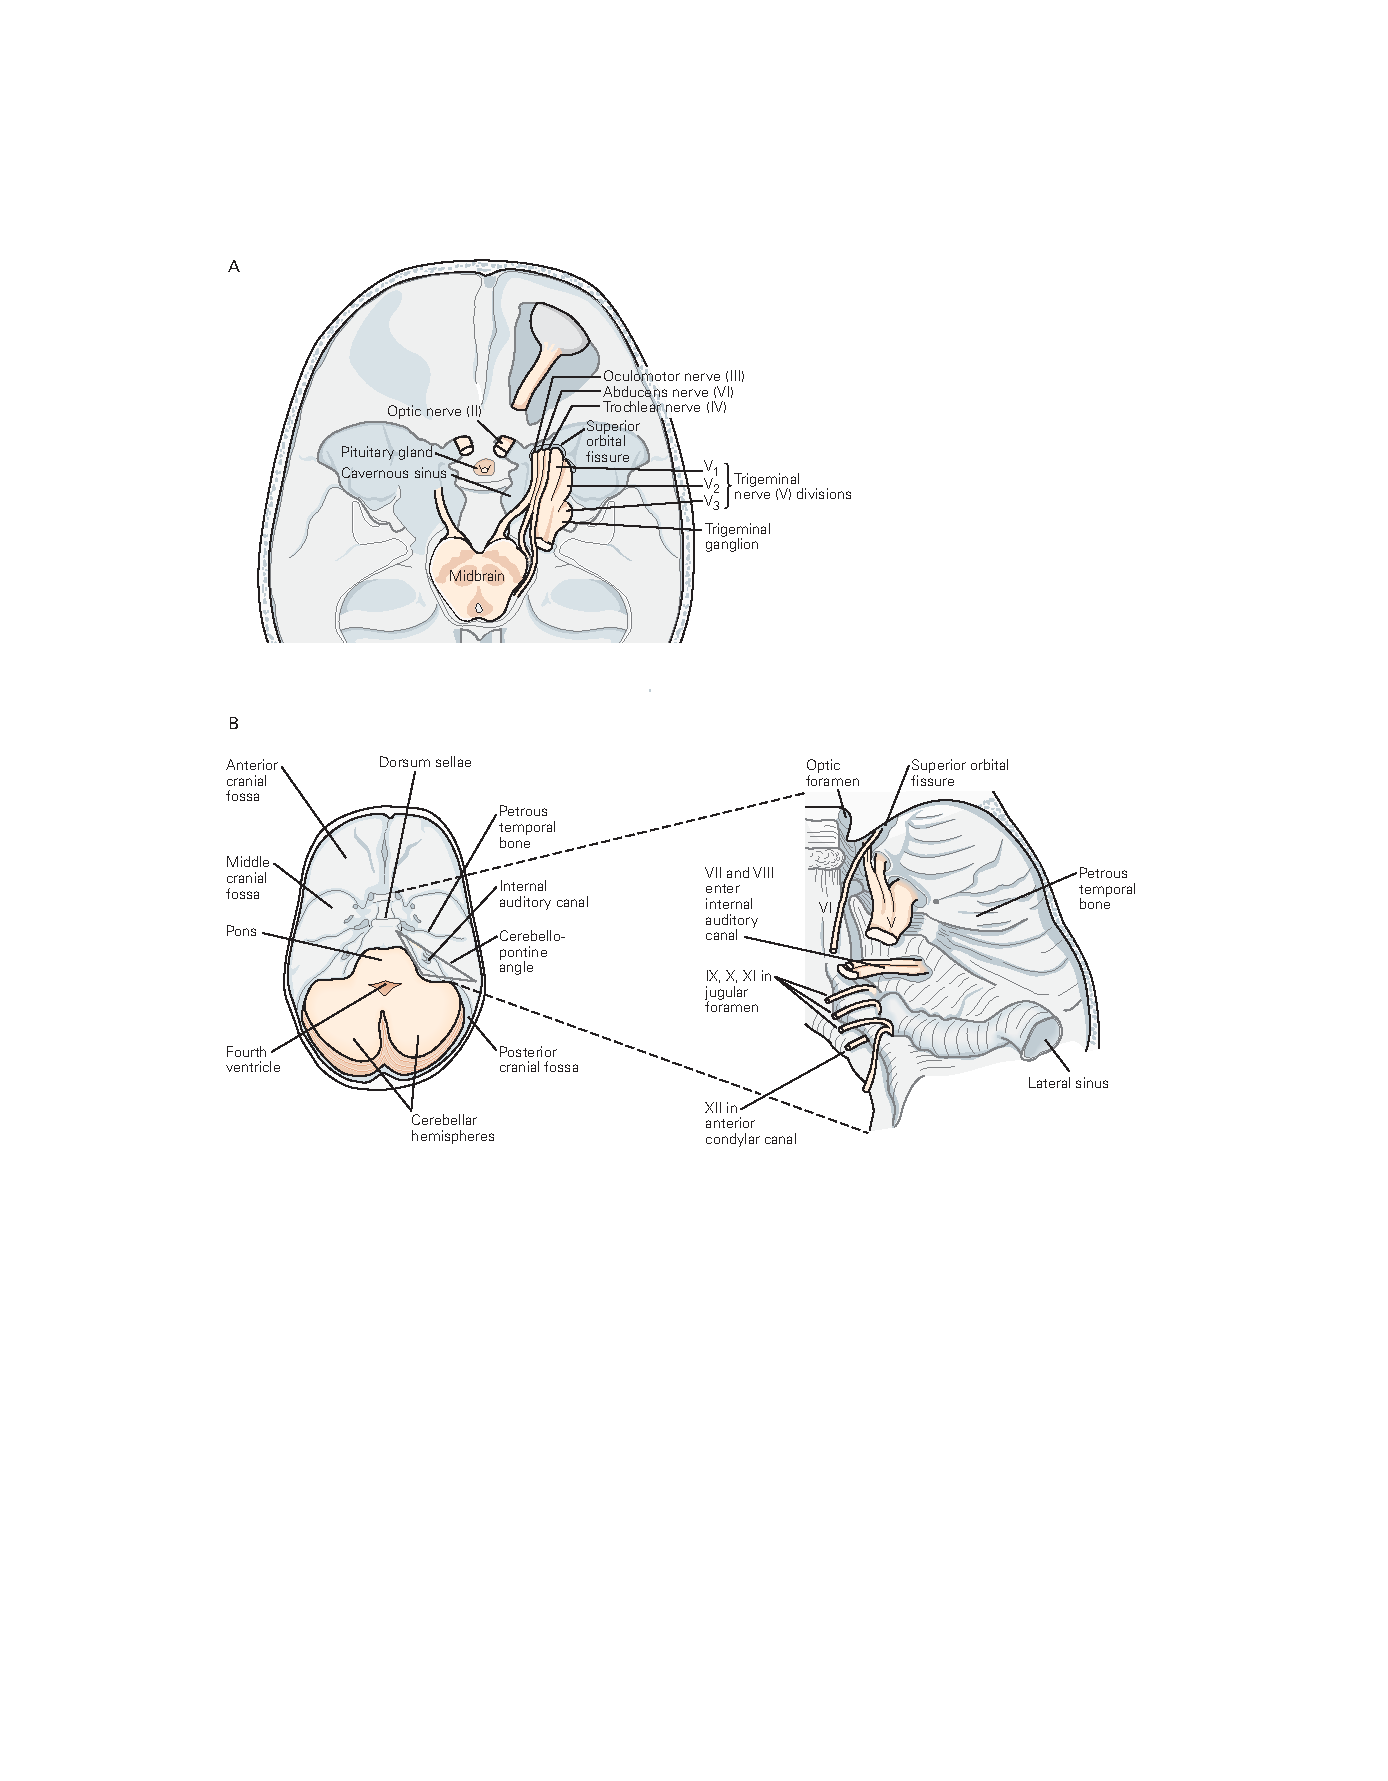
\includegraphics[width=1.0\linewidth]{chap40/fig_40_2}
	\caption{颅神经成群离开颅骨。
		\textbf{A.} 颅神经 II、III、IV、V 和 VI 在垂体窝附近离开颅骨。
		视神经 (II) 进入视神经孔,但动眼神经 (III)、滑车神经 (IV) 和外展神经 (VI) 以及三叉神经 (V) 的第一支从眶上裂离开。
		三叉神经的第二支和第三支分别穿过圆形和椭圆形的孔。
		\textbf{B.} 在后颅窝,面神经 (VII) 和前庭蜗神经 (VIII) 通过内耳道发出,而舌咽神经 (IX)、迷走神经 (X) 和副神经 (XI) 通过颈静脉孔发出。
		舌下神经 (XII) 有自己的孔。}
	\label{fig:40_2}
\end{figure}



与前脑相关的嗅觉 (I) 神经在第~\ref{chap:chap29}~章中有详细描述;
第~\ref{chap:chap21}~章和第~\ref{chap:chap22}~章描述了与间脑相关的视神经 (II) 。
脊髓副 (XI) 神经在解剖学上可以被认为是颅神经,但实际上是起源于较高的颈椎运动神经根的脊神经。
它向上进入颅骨,然后通过颈静脉孔出来,支配颈部的斜方肌和胸锁乳突肌。



\subsection{颅神经调节面部和头部的感觉和运动功能以及身体的自主功能}

三个眼部运动神经控制眼睛的运动。
外展神经 (VI) 的作用最简单;
它收缩外直肌以横向移动眼球。
滑车 (IV) 神经还支配一块肌肉,即上斜肌,它既可以压低眼睛,又可以根据眼睛的位置向内旋转。
动眼神经 (III) 供应眼眶的所有其他肌肉,包括眼睑牵开器。
它还提供负责瞳孔收缩的副交感神经支配,以响应光线和晶状体的调节以实现近距离视觉。
第~\ref{chap:chap35}~章详细讨论了眼动系统。


三叉神经 (V) 神经是一种混合神经(包含感觉轴突和运动轴突),它以两个根离开脑干。
运动根支配咀嚼肌(咬肌、颞肌和翼状肌)和上颚的一些肌肉(腭帆张肌)、内耳(鼓室张肌)和上颈部(下颌舌骨肌和二腹肌前腹)。
感觉纤维来自三叉神经节中的神经元,位于中颅窝的颅骨底部。


三叉神经节出现三个分支。
眼科 (V1) 与眼部运动神经一起穿过眶上裂(图~\ref{fig:40_2}A)以支配眼眶、鼻子、前额和头皮回到颅顶(图~\ref{fig:40_3})。
来自该部门的一些纤维还支配颅内前窝和中颅窝的脑膜和血管。
上颌骨支 (V2) 穿过蝶骨的圆孔,支配面颊和口腔上部的皮肤。
下颌骨分裂 (V3) 也包含三叉神经的运动轴突,通过蝶骨的卵圆孔离开颅骨。
它支配下巴、耳朵上方区域和口腔下部(包括舌头)的皮肤。


\begin{figure}[htbp]
	\centering
	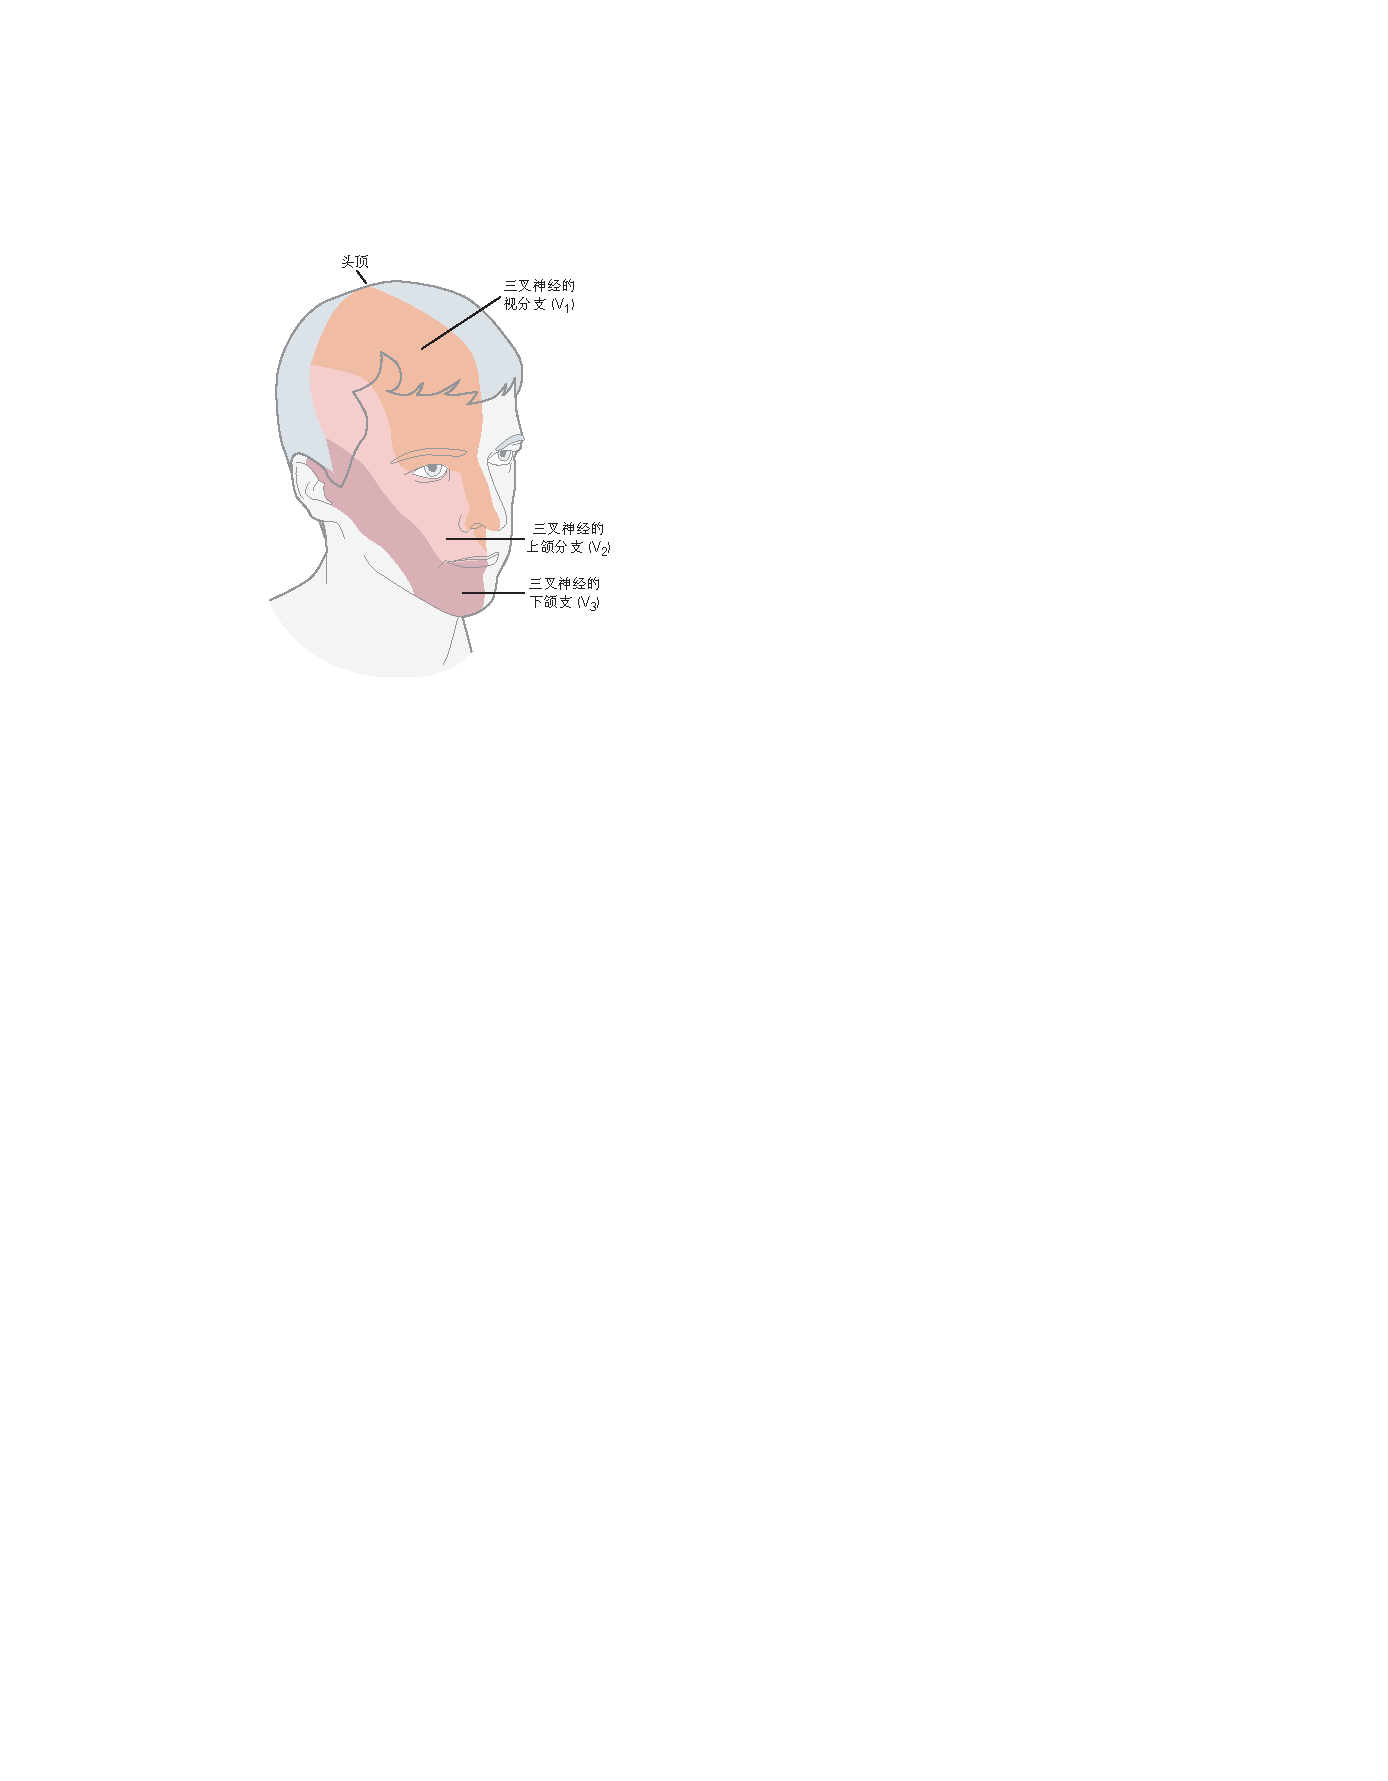
\includegraphics[width=0.4\linewidth]{chap40/fig_40_3}
	\caption{三叉神经 (V) 的三个感觉分支支配面部和头皮。
		V2 和 V3 部分还支配口腔的上部和下部,包括舌头。
		C2 颈根支配后脑勺。
		耳朵周围的区域由 VII 和 X 神经的分支支配。}
	\label{fig:40_3}
\end{figure}


完全的三叉神经感觉丧失导致整个面部和口腔内部麻木。
单侧三叉神经运动无力不会导致下颌闭合无力,因为两侧的咀嚼肌足以闭合下颌。
然而,当张开嘴巴时,下颌往往会偏向病变侧,这是因为对侧的翼内肌在没有抵抗力的情况下会将下颌拉向较弱的一侧。


面神经 (VII) 也是混合神经。
它的运动根支配面部表情的肌肉以及内耳的镫骨肌、茎突舌骨肌和上颈部二腹肌的后腹。
感觉根作为一个单独的束,即中间神经,穿过内耳道,起源于位于中耳附近的膝状神经节中的神经元。
在膝状神经节的远端,感觉纤维从运动支分叉。
一些神经支配外耳道的皮肤,而另一些则形成鼓索,它连接舌神经并从舌头的前三分之二传递味觉。
面神经的自主神经成分包括副交感神经纤维,这些纤维通过运动根到达蝶腭神经节和下颌下神经节,支配泪腺和唾液腺(腮腺除外)和脑血管系统。


面神经可能在贝尔麻痹中受到孤立的损伤,贝尔麻痹是某些病毒感染的常见并发症。
早期,由于病变侧肌肉无力,患者可能主要抱怨脸部向未受影响的一侧拉扯。
后来患侧嘴角下垂,食物从口中掉出,那一侧的眼睑不再闭合。
不眨眼可能会导致角膜干燥和受伤。 患者可能会抱怨声音在同侧耳朵中具有隆隆的音质,因为镫骨肌无法张紧听小骨以响应响亮的声音(镫骨反射)。
同侧舌头前三分之二的味觉也可能丧失。
如果贝尔麻痹是由膝状神经节的带状疱疹感染引起的,则可能会在外耳道(神经节的皮肤感觉区)中形成小水泡。


前庭耳蜗 (VIII) 神经包含来自两个神经节的两个主要感觉轴突束。
来自前庭神经节的纤维传递来自内耳半规管、椭圆囊和球囊的角加速度和线加速度的感觉。
来自耳蜗神经节的纤维传递来自耳蜗的有关声音的信息。
前庭神经鞘瘤是最常见的颅内肿瘤之一,可能沿着第 VIII 颅神经的前庭成分形成,因为它在内耳道内走行。 大多数患者只抱怨听力损失,因为大脑通常能够适应一侧前庭输入的逐渐丧失。


舌咽 (IX) 神经和迷走神经 (X) 是混合神经,为胸腔和内脏器官提供副交感神经自主输入。
这些密切相关的神经传递来自咽部和上呼吸道的感觉信息以及来自舌后三分之一和口腔的味觉信息。
舌咽神经传递来自颈部的内脏信息(例如,来自颈动脉体的血氧和二氧化碳信息,来自颈动脉窦的动脉压力信息),而迷走神经传递来自胸腹器官的内脏信息,除了 远端结肠和盆腔器官。
这两种神经都包括副交感神经运动纤维。
舌咽神经提供对腮腺唾液腺的副交感神经控制,而迷走神经支配颈部、胸部和腹部等其他内部器官。
舌咽神经仅支配上颚的一块肌肉,即茎突咽肌,它可以抬高和扩张咽部。
喉部和咽部其余的横纹肌受迷走神经控制。


迷走神经感觉神经元支配胃肠道的长度,因此能够调节多种餐后功能。
一个很好的例子是迷走神经传入神经在调节餐后食物摄入方面的作用。
\textit{胆囊收缩素}是十二指肠肠内分泌细胞在进食时分泌的一种内源性肽,有助于产生饱腹感。
\textit{胆囊收缩素}作用于(至少部分)肠道中的迷走神经传入神经,刺激饱腹感。
迷走神经的外源性电刺激现在在临床上用于治疗多种疾病,包括肥胖、顽固性癫痫,甚至抑郁症。
然而,这些影响背后的神经解剖学和分子机制仍然知之甚少。
同样,减肥手术仍然是最广泛使用和最有效的对抗肥胖的策略之一。
一些研究表明,手术改变迷走神经传入对肠道信号的反应性可能有助于这些手术后体重的持续减轻。


由于神经 IX 和 X 的许多功能是双侧的且部分重叠,因此神经 IX 的单侧损伤可能难以检测。
单侧颅神经X损伤患者声音嘶哑,因为一侧声带麻痹,吞咽可能有些困难。
口咽检查显示一侧上颚无力和麻木。


脊髓副 (XI) 神经是纯运动神经,起源于上颈脊髓的运动神经元。
它支配身体同一侧的斜方肌和胸锁乳突肌。
由于胸锁乳突肌的机械作用是将头部转向另一侧,因此左侧神经损伤会导致头部向右侧转向无力。
左侧大脑皮层的损伤会导致除胸锁乳突肌外整个右侧的随意肌无力;
相反,同侧胸锁乳突肌会变弱(因为左侧大脑皮层负责与世界右侧相互作用的肌肉,而左侧胸锁乳突肌将头部转向右侧)。


舌下神经 (XII) 也是纯粹的运动神经,支配舌头的肌肉。
当神经受伤时,例如在头颈癌手术期间,该侧的舌头会萎缩。
肌纤维表现出肌束抽搐(肌束震颤),通过舌头的薄粘膜可以清楚地看到。



\subsection{颅神经成群离开颅骨,常一起受伤}

在评估颅神经功能障碍时,重要的是要确定损伤是在脑内还是沿着神经走行更远。
由于颅神经通过特定的孔离开颅骨,这些位置的损伤会影响多条神经。


与眼眶感觉和眼球运动有关的颅神经——动眼神经、滑车神经和外展神经,以及三叉神经的眼科——沿着蝶鞍的外侧边缘聚集在海绵窦中, 然后通过与视神经孔相邻的眶上裂离开颅骨(图~\ref{fig:40_2}A)。
该区域的肿瘤,例如起源于脑垂体的肿瘤,通常首先通过对这些神经或相邻视交叉的压力来发现它们的存在。


颅神经 VII 和 VIII 在小脑桥脑角出脑干,脑干的外侧角在桥脑、延髓和小脑的交界处(图~\ref{fig:40_2}B),然后通过内耳道离开颅骨。
小脑桥脑角的常见肿瘤是前庭神经鞘瘤(有时被错误地称为“听神经瘤”),它起源于神经 VIII 前庭成分中的雪旺细胞。
小脑桥脑角的大肿瘤不仅会损害VII、VIII神经的功能,还会压迫V神经从小脑中脚出现的部位附近,引起面部麻木,或压迫小脑或其小脑脚 侧,造成同侧笨拙。


下颅神经(IX、X 和 XI)穿过颈静脉孔(图~\ref{fig:40_2}B),并且容易受到该部位肿瘤的压迫。
神经 XII 通过其自身的(舌下)孔离开颅骨,并且通常不受位于邻近颈静脉孔的肿瘤的影响,除非肿瘤变得非常大。
如果肿瘤累及第 IX 和 X 神经,但未累及第 XI 神经,则它通常位于脑干内或脑干附近,而不是靠近颈静脉孔。



\section{脑神经核团的组织遵循与脊髓的感觉和运动区域相同的基本计划}

脑神经核团组织成与脊髓的感觉和运动层同源的头尾柱(第~\ref{chap:chap18}~章和第~\ref{chap:chap31}~章)。
从产生脑干和脊髓的尾神经管的发育计划可以最好地理解这种模式。


胚胎尾神经管的横轴被限界沟、沿中央管、第四脑室和脑导水管侧壁的纵沟细分为翼板(背侧)和基底(腹侧)板(图~\ref{fig:40_4}))。
翼板形成脊髓背角的感觉组件,而基板形成腹角的运动组件。
中间灰质主要由协调脊髓反射和运动反应的中间神经元组成。


\begin{figure}[htbp]
	\centering
	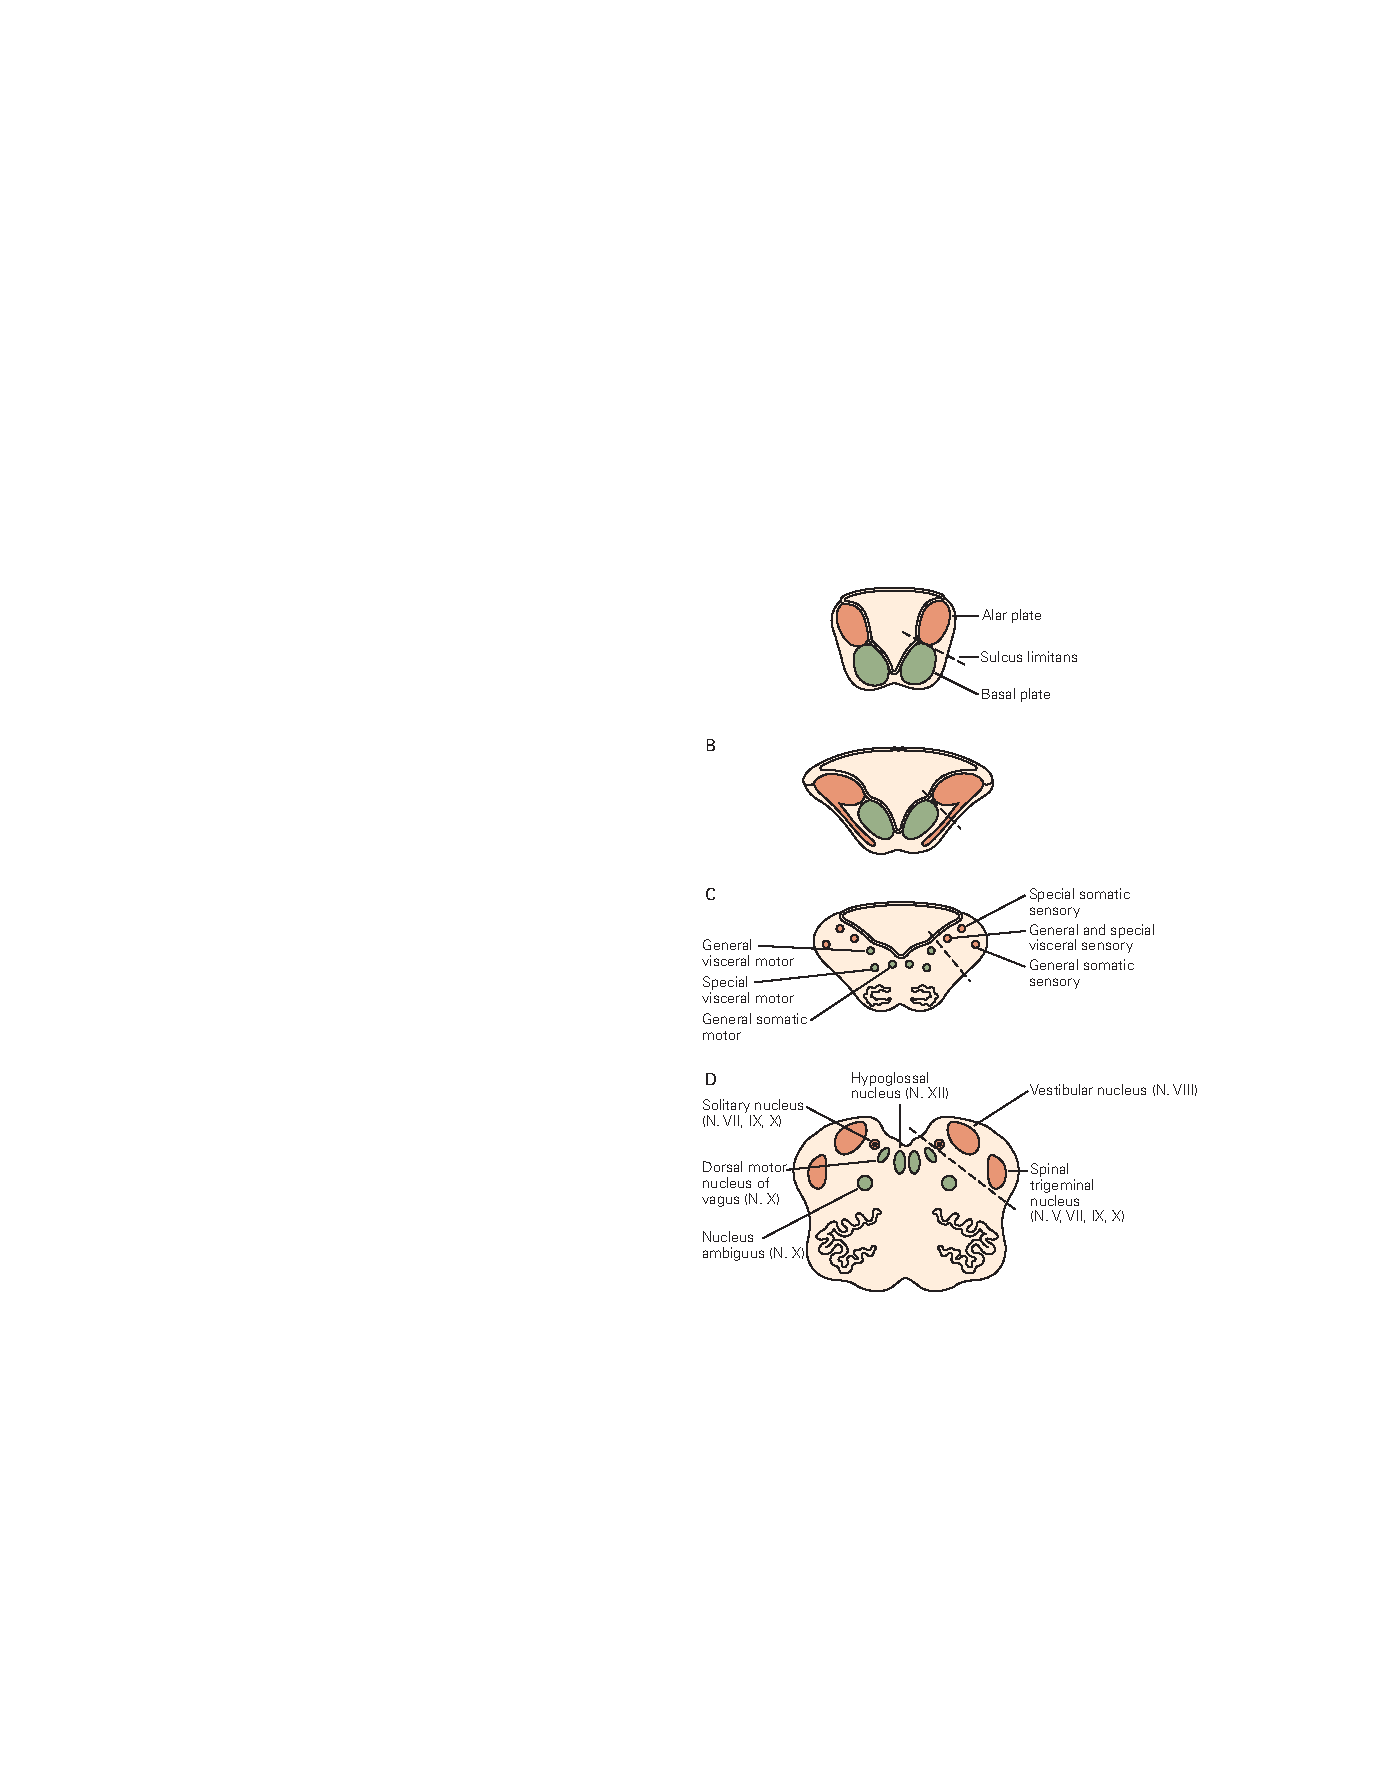
\includegraphics[width=0.6\linewidth]{chap40/fig_40_4}
	\caption{脑干的发育计划与脊髓的总体计划相同。
		\textbf{A.} 神经管被纵沟、界沟分为背侧感觉部分(翼板)和腹侧运动部分(基底板)。
		\textbf{B-D.} 在发育过程中,感觉细胞群和运动细胞群迁移到它们成年的位置,但在很大程度上保留了它们的相对位置。
		在成熟期(D 部分),在第四脑室壁和脑导水管中仍可识别到界沟(虚线),划分了背侧感觉(橙色)和腹侧运动(绿色)结构之间的边界。
		D 部分的部分来自延髓的延髓。}
	\label{fig:40_4}
\end{figure}


脑干共享这个基本计划。
当脊髓的中央管通向第四脑室时,神经管壁向外张开,使得背侧感觉结构(源自翼板)横向移位,而腹侧运动结构(源自基底 板)保持更内侧。
脑干的核团分为一般核团和特殊核团,其功能类似于脊髓椎板,特殊核团具有头部特有的功能,例如听觉、平衡、味觉和控制相关肌肉组织 到下巴、面部、口咽和喉部。



\subsection{胚胎脑神经核具有节段性组织}

尽管成年后脑中的感觉和运动核柱是按头尾排列的,但每个水平的神经元排列都源自早期胚胎中明显的分段模式。 
在神经元出现之前,神经板的未来后脑区域被细分为一系列大小大致相等的八个部分,称为菱形节(图~\ref{fig:40_5}A)。


\begin{figure}[htbp]
	\centering
	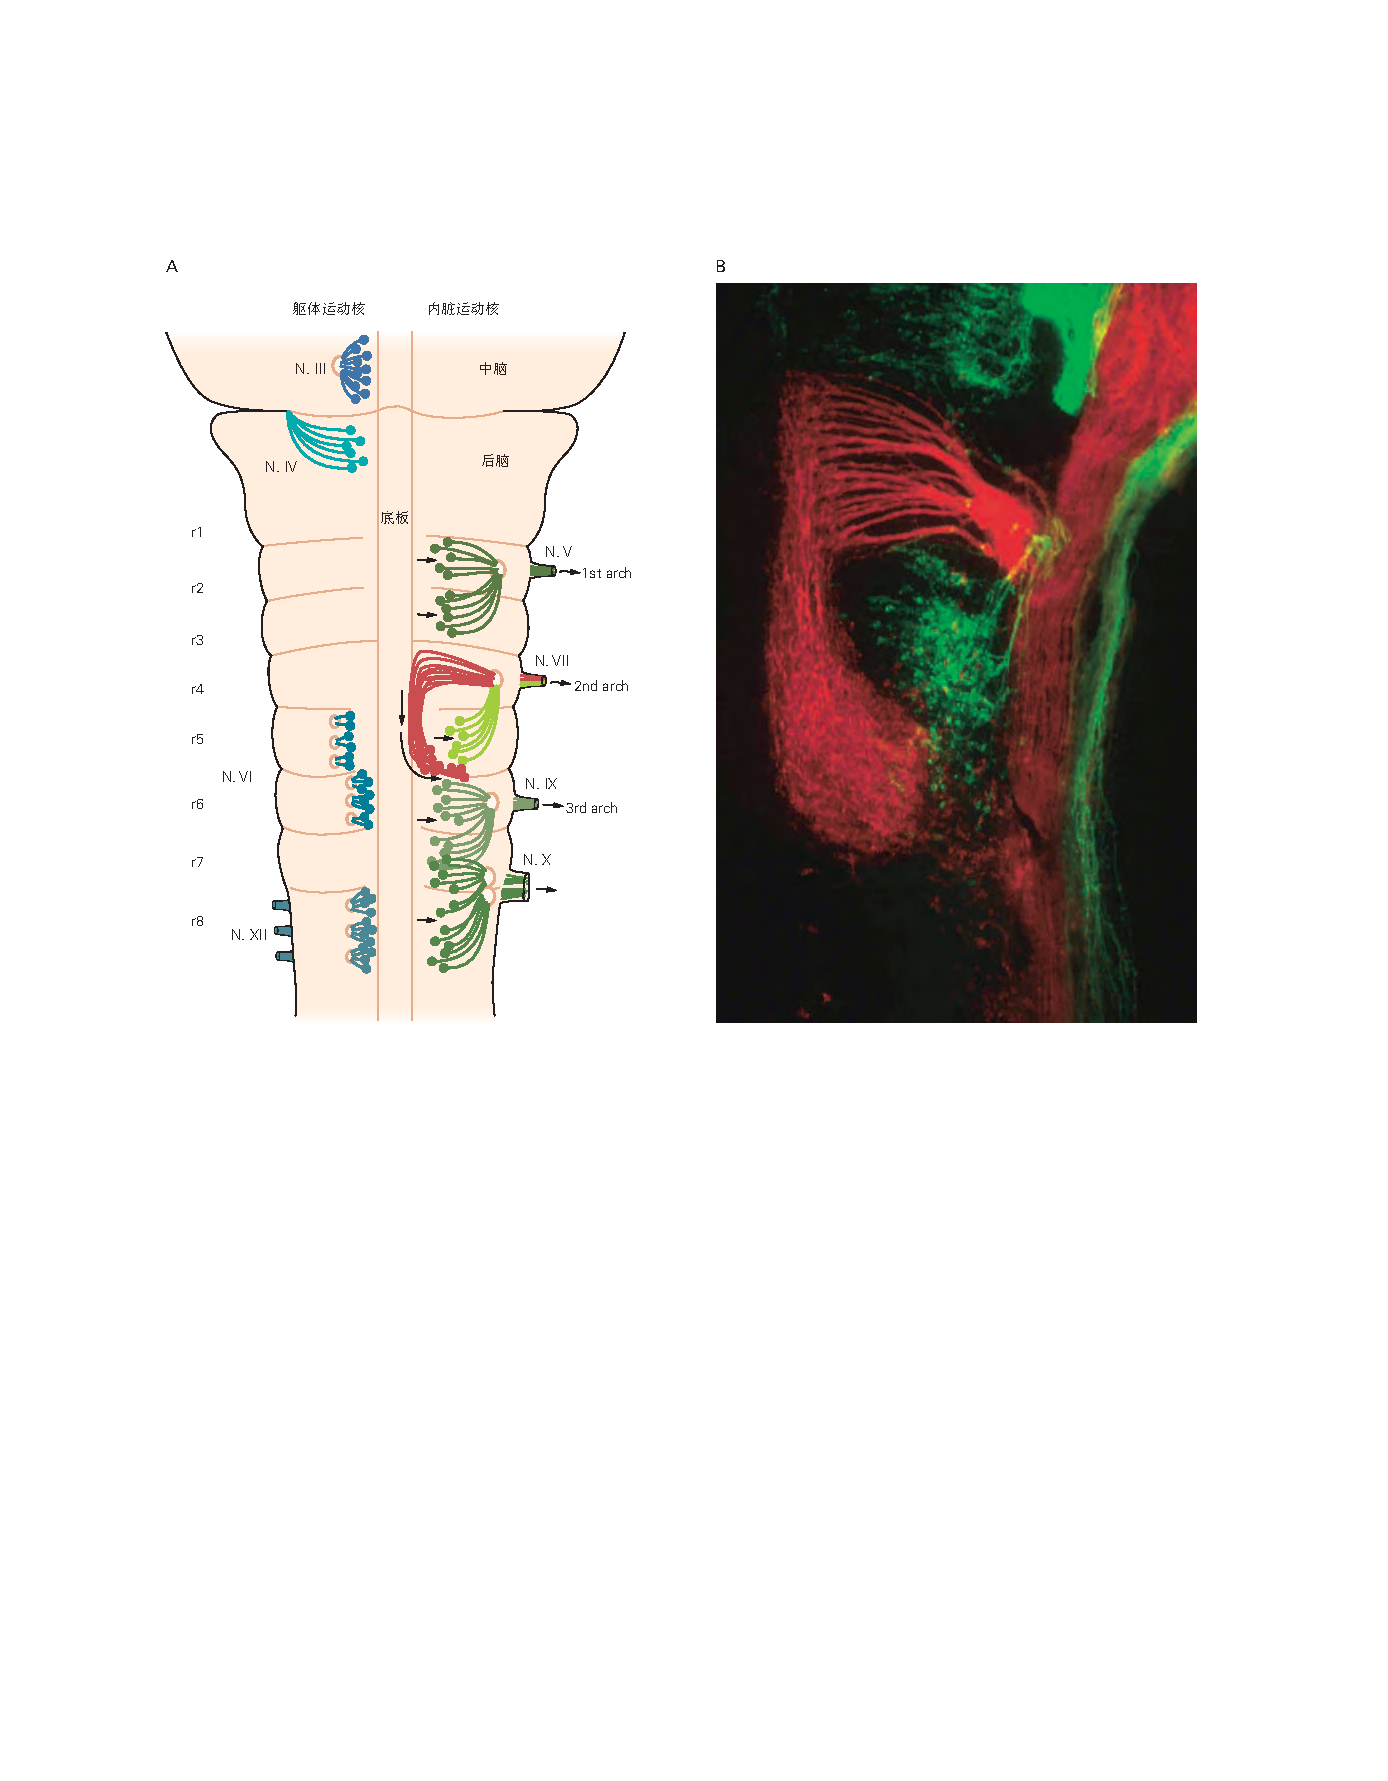
\includegraphics[width=1.0\linewidth]{chap40/fig_40_5}
	\caption{胚胎脑神经核团是分段组织的。
		\textbf{A.} 在发育中的后脑(此处从腹侧看),除菱形节 1 (r1) 外,每个后脑节段(菱形节)都形成了特殊和一般的内脏运动神经元(代表在脑干的右侧)。
		每个特殊的内脏运动核由两个菱形神经元组成:
		三叉神经运动核由 r2 和 r3 神经元组成,面神经核由 r4 和 r5 神经元组成,舌咽核由 r6 和 r7 神经元组成,舌咽神经核由 r6 和 r7 神经元组成, 由 r7 和 r8 中的神经元引起的迷走神经。
		这些核中每一个的神经元轴突在脑内横向走行,通过外侧神经上皮(r2、r4、r6 和 r7)的出口点离开大脑,并在脑外一起运行以形成各自的颅运动神经(V , VII, IX, X)。
		三叉神经 (V) 神经支配第一鳃弓的肌肉,面神经 (VII) 支配第二鳃弓的肌肉,舌咽 (IX) 神经支配第三鳃弓的肌肉。
		所有的内脏运动神经元(各种深浅不一的绿色,代表在脑干的右侧)最初在腹侧中线的底板旁边发育; 
		在将它们的轴突延伸到它们各自的出口点后,细胞体然后横向迁移(箭头)。
		例外是在 r4(红色)中形成的面部运动神经元;
		细胞体在向出口点延伸其轴突后,在横向迁移之前向尾端迁移到 r6 的轴向水平。
		与神经 VII(浅绿色)相关的一般内脏(副交感神经)运动神经元采取更传统的过程(见面板 B)。
		r1(滑车核)、r5 和 r6(外展核)以及 r8(舌下核)形成了一般躯体运动核(各种深浅不一的蓝色,代表在脑干的左侧)。
		这些神经元的细胞体仍然靠近它们的出生地,靠近底板。
		外展神经元和舌下神经元的轴突直接从腹侧离开大脑,没有横向走行。
		滑车神经元(浅蓝色)的轴突在脑内横向和背侧延伸,直到下丘尾部向内侧转动,在下丘后面交叉,并在对侧中线附近退出。
		\textbf{B.} 小鼠胚胎的脑干,其中荧光染料标记了不同的颅神经 VII 运动神经元群。
		一种红色荧光染料通过来自面神经运动根的逆行运输填充面部运动神经元的细胞体。
		这些神经元最初在 r4 中发育,然后沿着底板向后迁移到 r6(参见 A 部分中的红色神经元)。
		一种绿色荧光染料通过从中间神经根(感觉和神经节前一般内脏运动轴突)的逆行运输填充 r5 中一般内脏运动神经元的细胞体(见 A 部分中的浅绿色神经元)。}
	\label{fig:40_5}
\end{figure}


每个菱形节都发育出一组相似的分化神经元,就好像正在发育的后脑是由一系列模块组成的。
成对的菱形节与源自胚胎鳃弓的特定肌肉组相关(例如,菱形节 2 和 3 与咀嚼肌相关,菱形节 4 和 5 与面部表情肌相关)(图~\ref{fig:40_5}A)。
偶数菱形节先于奇数菱形节分化。
菱形节 2、4 和 6 分别形成三叉神经、面神经和舌咽神经的鳃运动核。
随后,菱形节 3、5 和 7 再次分别为这些核提供运动神经元;
在每种情况下,来自奇数菱形体的单个运动神经元的轴突在与偶数相邻菱形体的轴突连接时向嘴侧延伸。


在这个发育阶段,这些细胞核中的每一个都由来自两个相邻节段的同源神经元组成。
这种早期的横向节段组织在发育后期发生变化,因为菱形节边界消失,细胞体的背外侧迁移将细胞排列成头尾之间的柱。
最终,一些躯体和副交感神经运动神经元迁移到腹外侧被盖;
例如,菱形节 4 的面部运动神经元在外展核周围的迁移产生了面神经的内膝(图~\ref{fig:40_5}A)。
此外,来自每个菱形节的神经嵴细胞迁移到相应的鳃弓,在那里它们提供感觉和自主神经节细胞,以及弓肌发育的位置线索。



\subsection{成人脑神经核具有柱状组织}

总的来说,每侧的脑干核团被组织成六个头尾之间列,三个感觉核团和三个运动核团(图~\ref{fig:40_6})。
这些在后面考虑,从背外侧到腹内侧的顺序。
虽然这些柱子沿着脑干的头尾轴是不连续的,但具有相似功能(感觉或运动、躯体或内脏)的核团在脑干的每个水平都有相似的背外侧-腹内侧位置。


\begin{figure}[htbp]
	\centering
	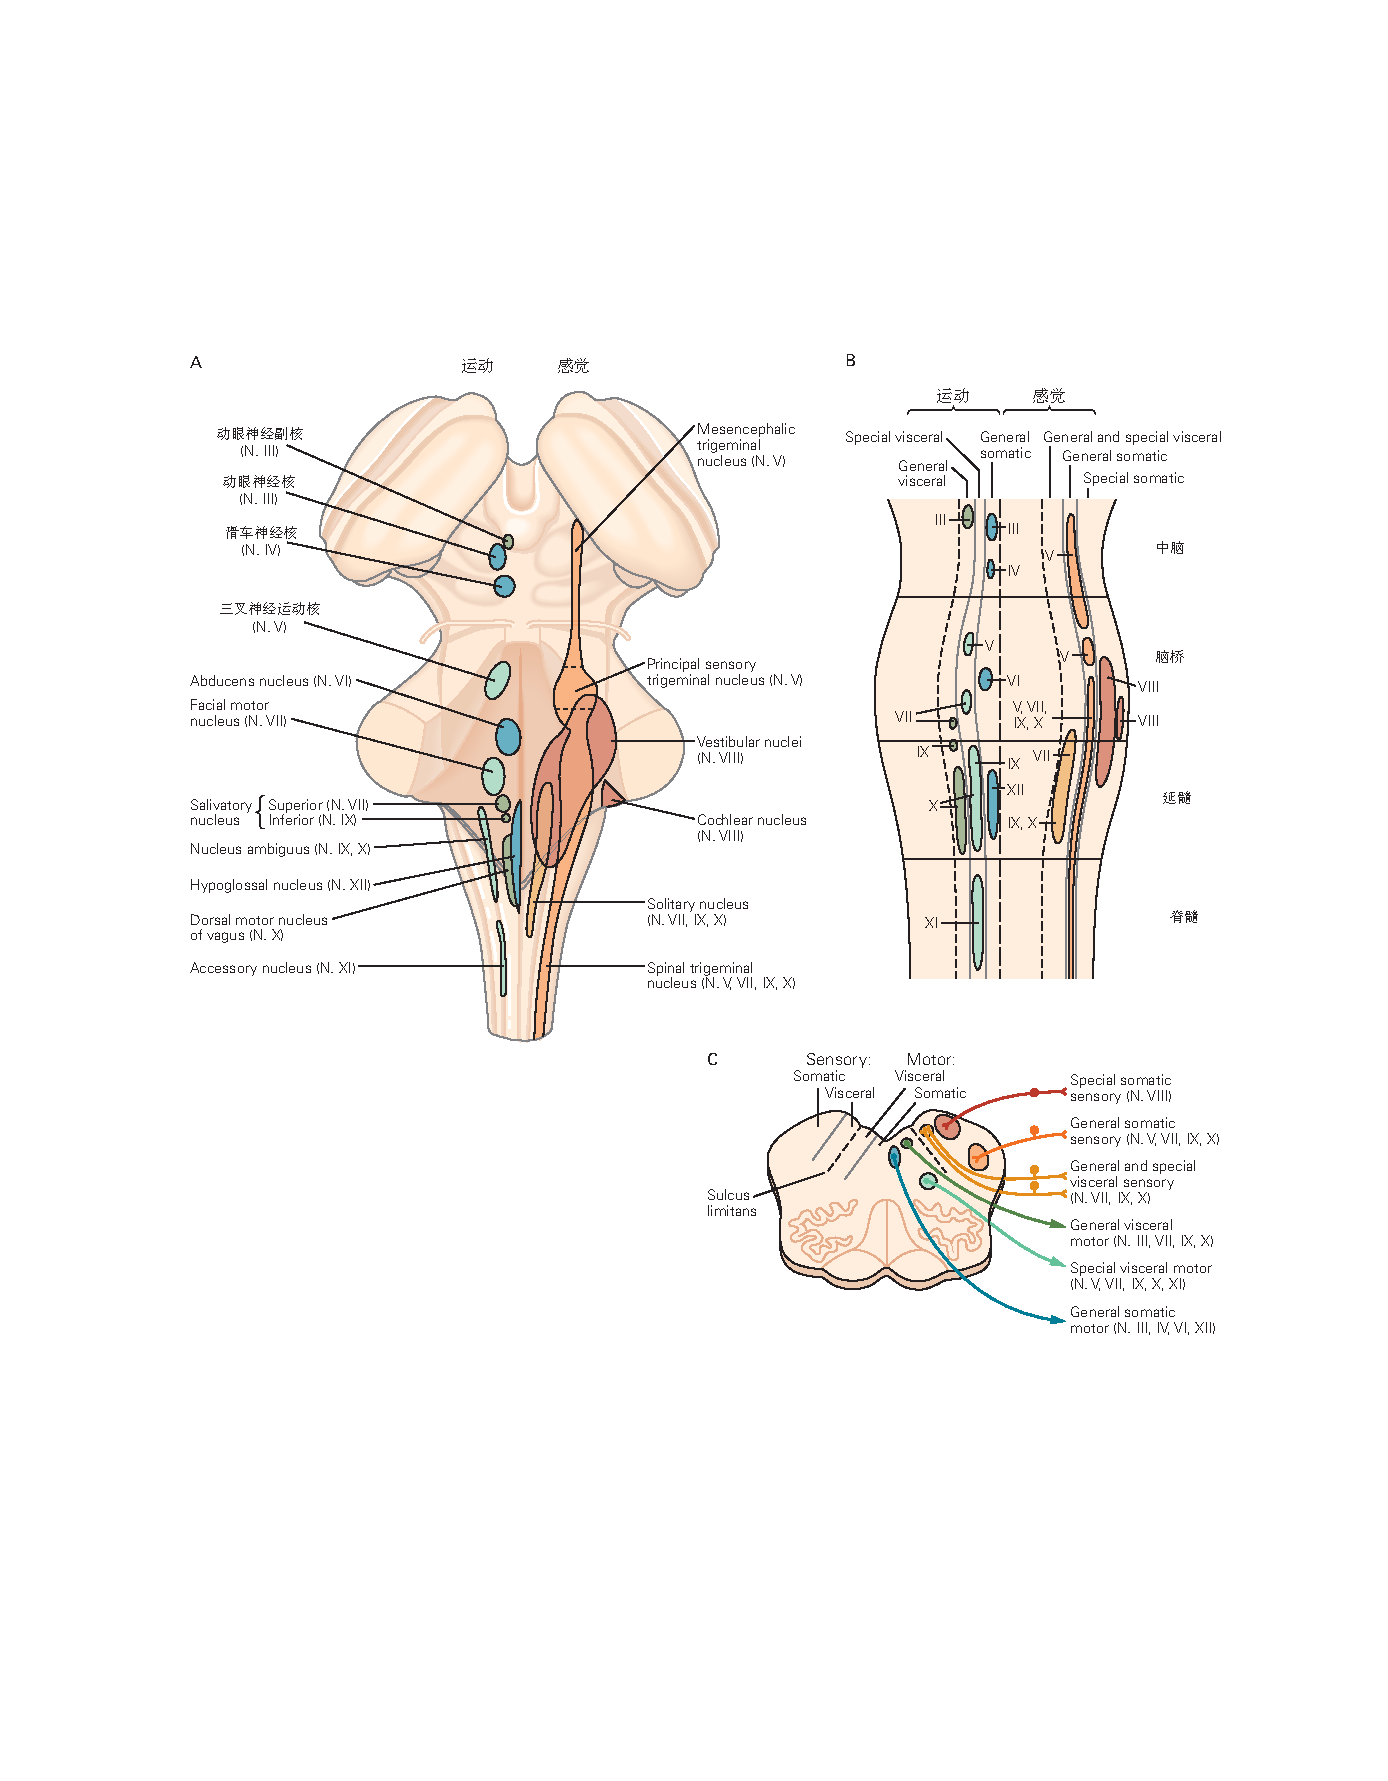
\includegraphics[width=1.0\linewidth]{chap40/fig_40_6}
	\caption{成人脑神经核团在脑干的头尾轴上分为六个功能柱。
		\textbf{A.} 这张人脑干的背面图显示了颅神经感觉核(右)和运动核(左)的位置。
		\textbf{B.} 脑神经核团的功能组织示意图更清楚地表明它们形成运动和感觉柱。
		\textbf{C.} 颅神经核的内侧-外侧排列显示在髓质水平的横截面中(与图~\ref{fig:40_4}D 比较)。}
	\label{fig:40_6}
\end{figure}


在每个运动核内,单个肌肉的运动神经元也排列成雪茄形纵柱。
因此,横截面中的每个运动核都形成了受神经支配区域的马赛克图。
例如,在面神经核的横截面中,支配不同面部肌肉的神经元簇形成了面部的地形图。


\textit{一般躯体感觉柱}

一般躯体感觉柱占据翼板的最外侧区域,包括三叉神经感觉核 (N. V)。
脊髓三叉神经核是脊髓背角最背层的延续(图~\ref{fig:40_5}A),有时也称为髓质背角。
沿着它的外表面是脊髓三叉神经束,它是脊髓\textit{背外侧束}的直接延续(第~\ref{chap:chap20}~章),因此允许一些颈部感觉纤维到达三叉神经核和一些三叉神经感觉轴突到达上颈段的背角。
这种安排允许背角感觉神经元具有比单个脊柱或三叉神经节段更广泛的输入范围,并确保三叉神经和上颈椎感觉图的整合。


脊髓三叉神经核接收来自三叉神经节 (N. V) 和所有与头部疼痛和温度有关的颅神经感觉神经节的感觉轴突,包括从外耳道传递信息的膝状神经节 (N. VII) 神经元,岩神经节 (N. IX) 细胞从上颚后部和扁桃体窝传递信息,结状神经节 (N. X) 轴突从咽后壁传递信息。
因此,脊髓三叉神经核代表整个口腔和面部表面。


脊髓三叉神经核中传入纤维的躯体组织是倒置的:前额位于腹侧,口腔区域位于背侧,舌头向内侧延伸至孤束核的味觉区,与孤束核共享一些传入信息 关于食物质地和温度。
来自脊髓三叉神经核的轴突在脑干的同一侧下降到颈脊髓,在那里它们与脊髓丘脑轴突在前连合处穿过中线并加入对面的脊髓丘脑束。
(由于这个原因,上颈脊髓损伤可能会导致面部麻木。)三叉神经丘脑轴突然后通过与脊髓丘脑束密切相关的脑干向后上升,为脑干核团提供反射运动和自主反应的输入,此外还携带 向丘脑传递疼痛和温度信息。


主要感觉三叉神经核位于桥中部,恰好位于三叉神经运动核的外侧。
它接收三叉神经节神经元的轴突,这些轴突与位置感和精细触觉辨别有关,这些信息与背柱从身体其他部位传递的感觉信息相同。
来自该核的轴突恰好在内侧丘系的背柱核的内侧束在一起,它们通过它们上升到腹后内侧丘脑。


中脑三叉神经核位于导水管周围灰质侧面的中脑水平,传递来自咀嚼肌和牙周韧带的机械感觉信息。
这个细胞核的大细胞不是中枢神经元,而是起源于神经嵴的初级感觉神经节细胞,与它们在三叉神经节中的亲属不同,它们在发育过程中迁移到大脑中。
这些伪单极细胞轴突的中央分支接触三叉神经运动核中的运动神经元,为下颌肌肉组织提供单突触反馈,这对于快速和精确控制咀嚼运动至关重要。


\textit{特殊躯体感觉柱}

特殊的躯体感觉柱有来自听神经和前庭神经的输入,并从翼板的中间区域发展而来。
耳蜗核 (N. VIII) 位于桥延髓交界处脑干的外侧边缘,接收来自耳蜗螺旋神经节的传入纤维。
耳蜗核的输出通过脑桥传递到上橄榄核和梯形核,并通过双侧传递到下丘(第~\ref{chap:chap28}~章)。
前庭核 (N. VIII) 更复杂。
它们包括四个不同的细胞群,它们将信息从前庭神经节传递到脑干、小脑和脊髓中的各个运动部位,这些部位与维持眼睛和头部运动的平衡和协调有关(第~\ref{chap:chap27}~章)。


\textit{内脏感觉柱}

内脏感觉柱与来自面部 (VII)、舌咽 (IX) 和迷走神经 (X) 的特殊内脏信息(味觉)和一般内脏信息有关。 它源自翼板中最内侧的神经元层。
来自这些来源的所有传入轴突都终止于孤束核。
孤束类似于脊髓三叉神经束或李绍尔束,将来自不同颅神经的传入神经束束在一起,因为它们沿着核的长度向尾部走行。
结果,来自内脏不同区域的感觉信息在细胞核中产生了内部身体的统一地图。


来自舌前三分之二的特殊内脏传入神经通过面神经的鼓索分支到达孤束核,而来自舌后部和口腔的神经传入神经则通过舌咽神经和迷走神经到达。
这些传入神经在孤束(或孤核)核的前三分之一处以粗略的躯体化方式终止。
一般内脏传入神经通过舌咽神经和迷走神经传递。
来自胃肠道其余部分(下至横结肠)的那些按地形顺序终止于孤核的中间部分,而来自心血管和呼吸系统的那些终止于尾部和侧部。


孤核直接投射到延髓和脊髓中的副交感神经和交感神经节前运动神经元,介导各种自主神经反射,以及协调自主神经和呼吸反应的网状结构部分。
大多数从孤核将信息从内脏传递到前脑的上行投射通过脑桥中的臂旁核传递,尽管有些直接到达前脑。
孤立核和臂旁核共同为下丘脑、基底前脑、杏仁核、丘脑和大脑皮层提供内脏感觉信息。


\textit{一般内脏运动专栏}

所有运动神经元最初都在底板附近发育,底板是神经管腹侧中线的一条纵向非神经元细胞带(第~\ref{chap:chap45}~章)。
注定要成为三种类型的脑干运动神经元的神经元背外侧迁移,安置在三个不同的头尾柱中。
形成一般内脏运动柱的神经元沿着基板的最外侧区域占据一个位置,就在沟界的内侧。
在发育过程中,注定要加入上唾液核(面神经的一部分)和疑核(迷走神经的一部分)的副交感神经运动神经元向腹外侧迁移,留下轴突在向外侧转动离开脑干之前向内侧上升,在 类似于面部运动神经元的过程。


\textit{动眼神经副核} (N. III) 位于将躯体动眼神经元分开的中线,恰好位于大脑导水管底部下方。
它包含节前神经元,通过睫状神经节控制瞳孔收缩和晶状体调节。


上唾液核 (N. VII) 位于面部运动核的背侧,由副交感神经节前神经元组成,这些神经节前神经元支配舌下和下颌下唾液腺和泪腺,并通过蝶腭和下颌下副交感神经节进行颅内循环。


与胃肠道相关的副交感神经节前神经元在髓质水平形成一个柱,正好位于舌下神经核的背侧和孤束核的腹侧。
在该柱的最前端是下唾液核 (N. IX),它包含通过耳神经节支配腮腺的神经节前神经元。
该列的其余部分构成背侧运动迷走神经核 (N. X)。
该核中的大部分节前神经元支配横膈膜下方的胃肠道;
少数是心脏运动神经元。


疑核 (N. X) 贯穿延髓腹外侧的长尾端,包含支配胸腔器官(包括食道、心脏和呼吸系统)的副交感神经节前神经元,以及支配横纹肌的特殊内脏运动神经元 喉部和咽部,以及产生呼吸运动模式的神经元(见本章后面部分)。
副交感神经节前神经元以地形学方式组织,食道最靠近头侧和背侧。


\textit{特殊内脏运动专栏}

特殊的内脏运动柱包括支配来自鳃(咽)弓的肌肉的运动核。
因为这些弓与鱼的鳃同源,所以这些肌肉被认为是特殊的内脏肌肉,尽管它们是横纹的。
在发育过程中,这些细胞群迁移到基板的中间位置,最终位于被盖的腹外侧。


三叉神经运动核 (N. V) 位于脑桥中部水平并支配咀嚼肌。
附近位于独立的簇中的是支配鼓室张肌、腭帆张肌和下颌舌骨肌以及二腹肌前腹的三叉神经副核。


面部运动核 (N. VII) 位于脑桥尾部水平的三叉神经运动核的尾部,并支配面部表情的肌肉。
在发育过程中,面部运动神经元在向外侧、腹侧和尾侧转向它们在桥延髓交界处的最终位置之前,在外展核的内侧边缘向内侧和嘴侧移动(图~\ref{fig:40_5}A)。
轴突留下的这条蜿蜒曲折的路线形成了面神经的内膝。
相邻的副面部运动核支配茎突舌骨肌和镫骨肌以及二腹肌的后腹。


疑核包含带有轴突的鳃运动神经元,这些轴突在舌咽神经和迷走神经中运行。
这些神经元支配喉部和咽部的横纹肌。
在发育过程中,这些运动神经元迁移到延髓腹外侧,因此,它们的轴突向背内侧运动迷走神经核移动,然后在延髓内急剧转向横向退出,类似于面部运动轴突的过程。


\textit{通用躯体运动专栏}

躯体运动柱的神经元在发育过程中迁移最少,保持靠近腹侧中线。
动眼神经核 (N. III) 位于中脑水平;
它由支配内侧、上、下直肌、下斜肌和提眼睑的五个运动神经元柱组成。
内直肌、下直肌和下斜肌的运动神经元位于脑干神经发出的一侧,而上直肌的运动神经元则位于对侧。
提肌运动神经元是双侧的。


神经支配滑车肌的滑车核 (N. IV) 位于中脑/桥脑喙部水平,与神经出口相对的脑干一侧。
支配外直肌的外展核 (N. VI) 位于桥中部水平。
髓质中的舌下神经核 (N. XII) 由几列神经元组成,每列神经元支配舌头的一块肌肉。



\subsection{脑干的组织在三个重要方面不同于脊髓}

脑干组织和脊髓组织之间的一个主要区别是,许多沿着脊髓外部延伸的长的上升和下降感觉束被并入脑干内部。
因此,上行感觉束(内侧丘系和脊髓丘脑束)穿过脑干的网状结构,听觉、前庭和内脏感觉通路也是如此。


第二个主要区别是在脑干中,小脑及其相关通路形成附加结构,叠加在脊髓的基本结构上。
小脑束和核的纤维与锥体和锥体外系运动系统的纤维束在一起,形成脑干的大腹侧部分。
因此,从中脑到延髓,脑干分为背侧部分,即被盖,遵循脊髓的基本节段计划,以及腹侧部分,其中包含与小脑和下行运动相关的结构路径。
在中脑水平,腹侧(运动)部分包括大脑脚、黑质和红核。
脑桥的基底包括脑桥核、皮层脊髓束和小脑中脚。
在髓质中,腹侧运动结构包括锥体束和下橄榄核。


第三个主要区别是,虽然后脑在发育过程中被分成菱形节,但在成年大脑中没有明确的重复模式。
相比之下,脊髓在发育过程中并未分段,但最终模式由重复的分段组成。
腹根轴突和背根神经节突出的阶梯状排列表明,分割是由相邻身体节段或它们迁移到的体节的极化效应强加的——在每个体节中,喙部吸引轴突生长锥和神经嵴 细胞,而尾部是排斥的。
在头部,这种模式是缺乏的,因为颅中胚层没有被分割成体节,而是在菱形节的影响下发展。



\section{脑干网状结构中的神经元群协调稳态和生存所需的反射和简单行为}

19 世纪,\textit{查尔斯$\cdot$达尔文}在他的《人与动物的情绪表达》一书中指出,在相似的情绪情况下(恐惧、愤怒、厌恶、快乐),所有哺乳动物的面部表情肌肉都会以相似的模式被激活。
他假设面部表情的模式一定深深植根于脑干的组织中。
我们现在认识到,广泛的反射和简单、重复、协调的行为,例如面部情绪表达、呼吸和进食,是由脑干网状结构中称为模式发生器的神经元控制的,这些神经元会产生刻板的先天反应。
神经系统疾病患者的颅神经反射和运动模式受损可以指示脑干损伤的准确部位。



\subsection{颅神经反射涉及单突触和多突触脑干中继}

瞳孔对光的反应(瞳孔光反射)由瞳孔扩张肌中的交感神经张力和虹膜瞳孔收缩肌中的副交感神经张力之间的平衡决定。
交感神经张力由颈上神经节中的节后神经元维持,而颈上神经节又由第一和第二胸椎节段中的节前神经元支配。
副交感神经张力由在\textit{动眼神经副核}和中脑邻近区域的节前神经元控制下的节后睫状神经节细胞提供。


照射在视网膜上的光会激活一类特殊的视网膜神经节细胞,它们充当亮度检测器。
这些细胞接收来自含有感光色素的视杆细胞和视锥细胞的输入,但它们也有自己的感光色素黑视蛋白,即使视杆细胞和视锥细胞退化,它们也能对光做出反应。
这些细胞将它们的轴突通过视神经、交叉和视束传送到橄榄前顶核,在那里它们终止于神经元,这些神经元的轴突投射到\textit{动眼神经副核}中的节前神经元(图~\ref{fig:40_7})。
因此,后连合区域中脑背侧的损伤可以防止瞳孔光反应(中位,固定瞳孔),而动眼神经损伤消除了该瞳孔的副交感神经张力(固定和散大的瞳孔)。
含有黑视蛋白的视网膜神经节细胞也投射到下丘脑的视交叉上核,在那里它们将昼夜节律带入昼夜循环(第~\ref{chap:chap44}~章)。


\begin{figure}[htbp]
	\centering
	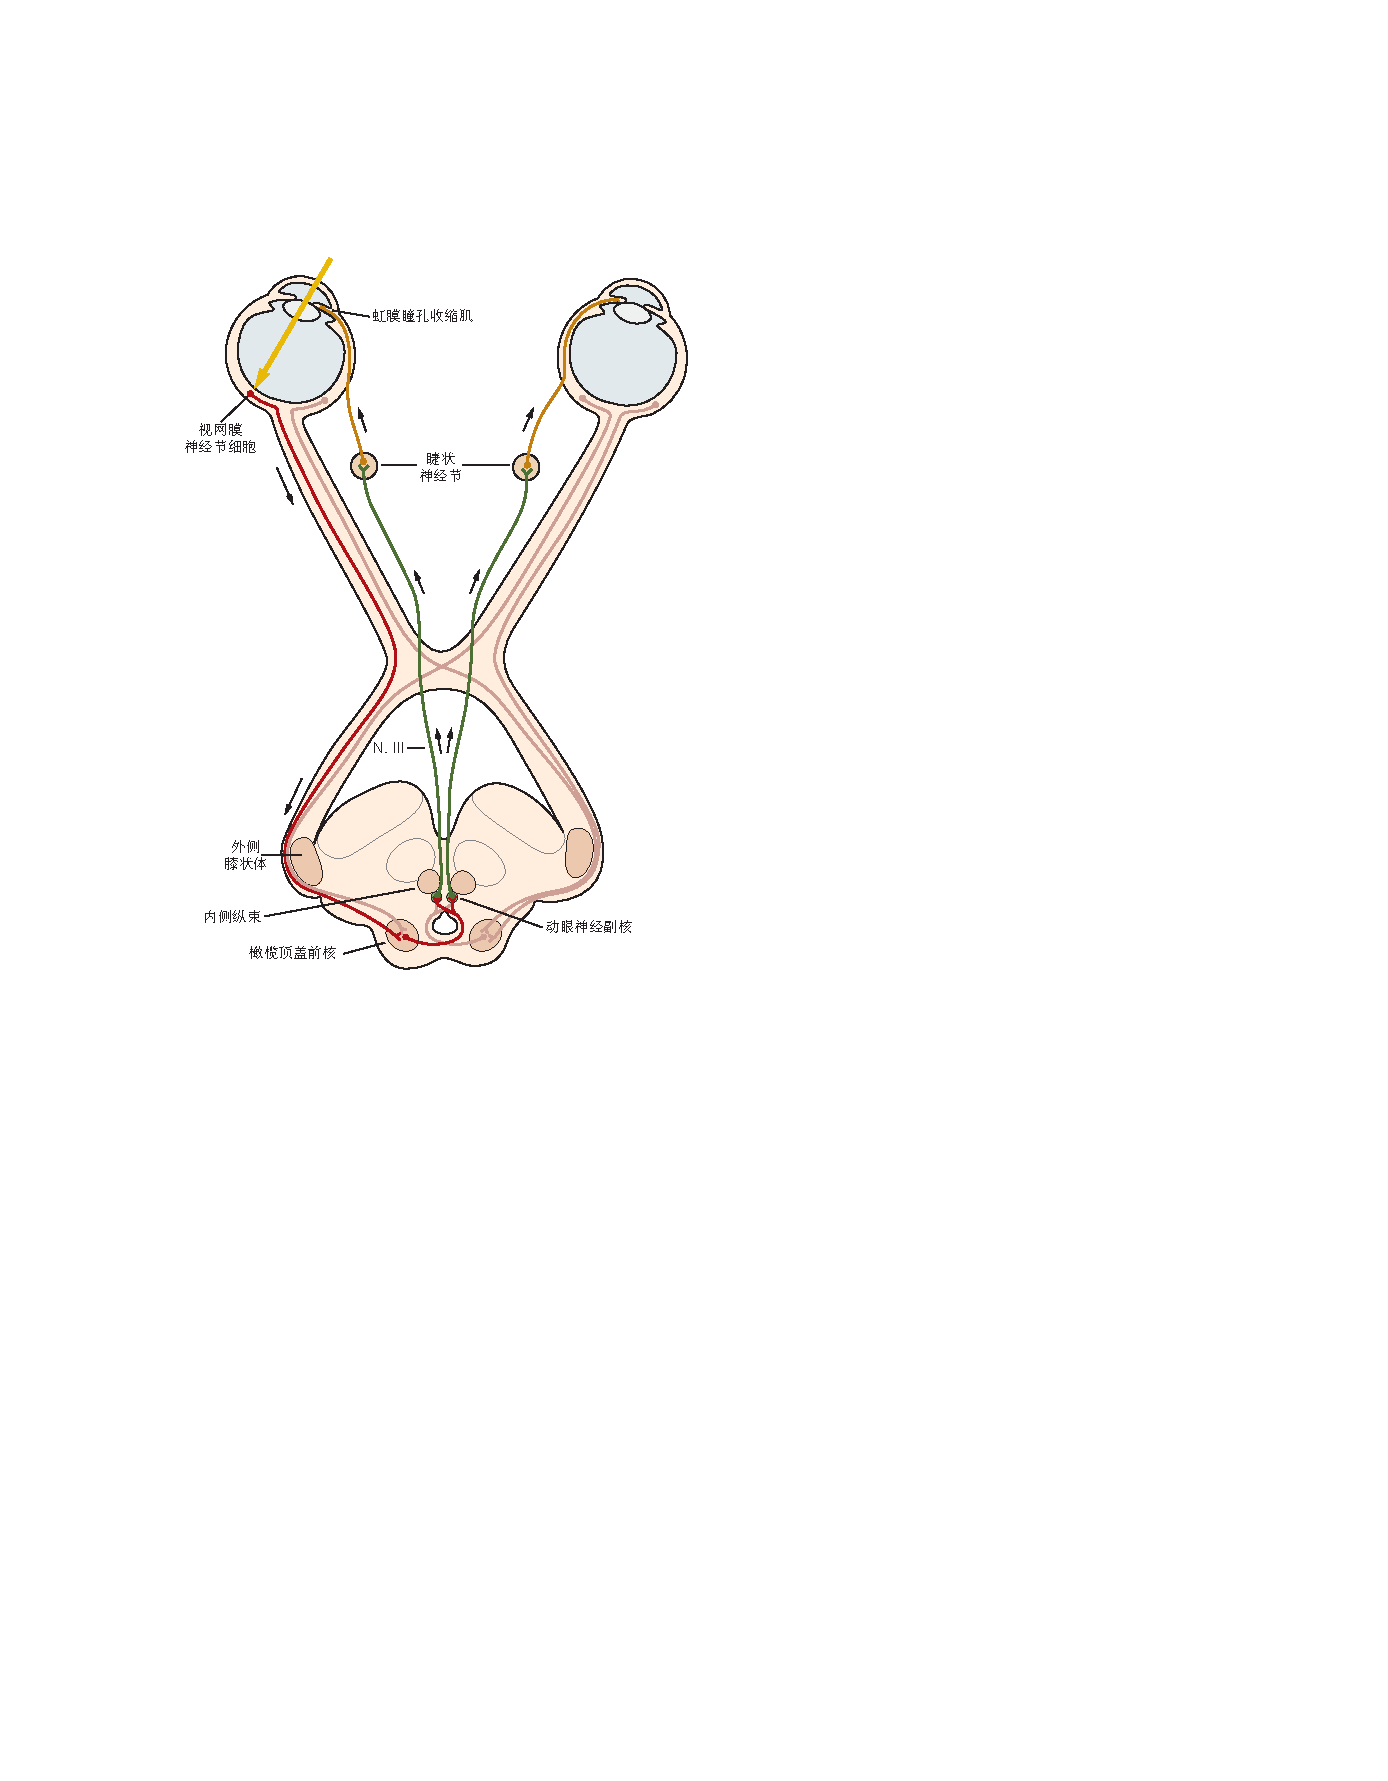
\includegraphics[width=0.6\linewidth]{chap40/fig_40_7}
	\caption{瞳孔对光的反应是由虹膜的副交感神经支配介导的。
		含有感光色素黑视蛋白的视网膜神经节细胞充当亮度探测器,将它们的轴突通过视束发送到位于中脑和丘脑交界处的橄榄核。
		该核中的神经元通过后连合投射到\textit{动眼神经副核}内和周围的副交感神经节前神经元。
		节前细胞的轴突与动眼神经 (III) 一起退出并接触睫状神经节细胞,睫状神经节细胞控制虹膜中的瞳孔收缩肌。}
	\label{fig:40_7}
\end{figure}


在头部运动期间,前庭眼反射通过与头部旋转相反的方向旋转眼球来稳定视网膜上的图像。
这些反射被从前庭神经节和神经到内侧、上和外侧前庭核的通路激活,并从那里到网状结构中的神经元和协调眼球运动的眼球运动核。
反射运动在昏迷患者中最为明显,在这些患者中转动头部会引起眼睛的反向旋转运动(所谓的娃娃眼运动)。
脑桥中这些通路的损伤会损害这些运动。


当轻轻刺激角膜(例如,用一缕棉花)时,角膜反射包括双眼睑闭合以及眼睛向上转动(贝尔现象)。
来自三叉神经第一部分的感觉轴突终止于脊髓三叉神经核,三叉神经核将感觉信号传递给与面部运动核相邻的网状结构中的模式发生器神经元。
模式发生器神经元向运动神经元提供双侧输入,运动神经元通过使眼轮匝肌闭合眼睑和动眼神经核使眼睛在眼眶中向上和向后滚动来保护角膜免受损伤。
由于模式发生器的输出是双侧的,因此感觉通路的损伤会阻止双眼的反射,而面神经的损伤只会阻止同一侧的闭合。


镫骨反射收缩镫骨肌以响应响亮的声音,从而抑制小骨的运动。
感觉通路通过耳蜗神经和神经核到达与面部运动核相邻的网状结构,然后从那里到达在面神经中运行的镫骨运动神经元。
如前所述,在面神经损伤的患者中(例如,贝尔麻痹),镫骨反射受损,并且患者主诉该耳中的声音具有“轰鸣”音质(听觉过敏)。


多种胃肠道反射由多突触脑干中继控制。
例如,品尝食物会导致孤核中的神经元投射到邻近运动面部和背侧运动迷走神经核的网状结构,从而刺激节前唾液腺神经元。
食物在嘴里的接触也会引起胃收缩和胃酸分泌,这可能是通过孤核直接输入迷走神经背核中的副交感神经节前胃神经元。
在患有贝尔麻痹的患者中,受损的 VII 神经副交感神经轴突可能会异常再生,从而导致唾液腺轴突错误地到达泪腺,导致美味食物引发反射性流泪(鳄鱼泪)。


咽反射保护气道以响应口咽后部的刺激。
舌咽神经和迷走神经中的传入感觉纤维终止于脊髓三叉神经核,其轴突投射到与疑核相邻的网状结构。
疑核中的鳃运动神经元支配咽后部肌肉,导致上颚抬高、咽部肌肉收缩(以排出有害刺激)和气道关闭。 喉咙一侧的呕吐反射消失表明该侧的髓质或颅神经 X 受损(颅神经 IX 在咽部具有如此小的感觉和运动神经支配区域,因此横断该神经不会引起 明显的赤字)。



\subsection{模式发生器协调更复杂的刻板行为}

正如达尔文所提出的,靠近面核的网状结构中的模式发生器神经元池通过面部两侧面部肌肉同时收缩的刻板模式来控制面部情绪表达。
脑干两侧的模式发生器神经元投射到大脑两侧的面部运动神经元,因此自发的面部表情几乎总是对称的。
即使是脑半球严重中风并且不能自主移动对侧口面部肌肉的患者,在听到笑话时仍然倾向于对称地微笑,并且可以对称地扬起眉毛,这两者都是由面部模式生成器启动的。


类似地,与进食有关的口面部运动是由调节行为的颅运动核附近网状结构中的模式发生器神经元产生的。
舔运动组织在靠近舌下核的网状结构中,靠近三叉神经运动核的咀嚼运动,靠近面部和疑核的吸吮运动,以及靠近疑核的吞咽运动。
毫不奇怪,这些网状区域中的神经元彼此紧密相连,并从与味觉有关的孤束核部分和与舌头和口腔感觉有关的脊髓三叉神经核部分以及来自 相邻网状结构中的神经元对食物的味道、质地和温度的更复杂组合做出反应。
因此,即使是去大脑的老鼠也能做出适当的选择,选择吞咽和拒绝哪些食物。


呕吐是由模式发生器神经元介导的协调反应的另一个例子。
血流中的有毒物质可以被后区的神经细胞检测到,该区是沿着第四脑室底部与孤束核相邻的一个小区域。
与大多数受血脑屏障保护的大脑不同,最后区包含有孔的毛细血管,使其神经元能够对血流中的内容物进行采样。
当这些神经元检测到毒素时,它们会激活腹外侧延髓中的神经元池,这些神经元控制一种反应模式,清除消化道中的任何有毒物质。
这些反应包括胃和食道蠕动的逆转、腹部肌肉收缩的增加以及呕吐反射中使用的相同运动模式的激活以清除口咽部不需要的物质。


由脑干组织的各种反应需要颅运动模式与自主反应(有时是内分泌反应)的协调。
一个很好的例子是压力感受器反射,它确保足够的血液流向大脑(第~\ref{chap:chap41}~章)。
孤束核通过迷走神经 (X) 接收有关主动脉弓伸展的信息,并通过舌咽 (IX) 神经接收有关颈动脉窦伸展的信息。
该信息被传递到腹外侧髓质中的神经元,这些神经元会产生协调反应,保护大脑免受血压下降的影响。


主动脉弓和颈动脉窦的拉伸减少减少了对疑核中副交感神经节前心脏迷走神经元的驱动,导致迷走神经张力降低和心率增加。
同时,延髓头侧腹外侧神经元的放电增加会驱动交感神经节前血管收缩神经元和心脏加速神经元。
这种增加的心输出量和增加的血管阻力的结合使血压升高。
同时,延髓腹外侧的其他神经元会增加下丘脑神经元的放电,这些神经元会从垂体后叶的末梢分泌血管加压素。
加压素也有直接的血管收缩作用,它通过减少肾脏的水排泄来维持血容量。



\subsection{呼吸控制提供了模式发生器如何集成到更复杂行为中的示例}

脑干最重要的功能之一是控制呼吸。
在人类妊娠 11 至 13 周的子宫内,脑干会自动产生呼吸运动,并从出生到死亡不间断地持续。
这种行为不需要任何有意识的努力,事实上,我们甚至很少想到需要呼吸。
呼吸的主要目的是使肺部通气以控制血液中氧气、二氧化碳和氢离子的水平。
(这些通常在临床上一起测量并称为“血气”。)呼吸运动涉及膈肌收缩,由膈神经激活。
膈肌在必要时由辅助呼吸肌辅助,包括肋间肌、咽肌(改变气道直径)、一些颈部肌肉(帮助扩张胸部)、舌突出肌(打开气道),甚至 一些面部肌肉(使鼻孔张开)。


呼吸活动可以由髓质产生,即使它与神经系统的其余部分隔离。
许多髓质神经元具有与吸气或呼气相关的放电模式(图~\ref{fig:40_8}A)。
有些具有更精致的模式,例如仅在早期灵感或晚期灵感时触发。
这些呼吸神经元集中在两个区域,即背侧和腹侧呼吸组。


\begin{figure}[htbp]
	\centering
	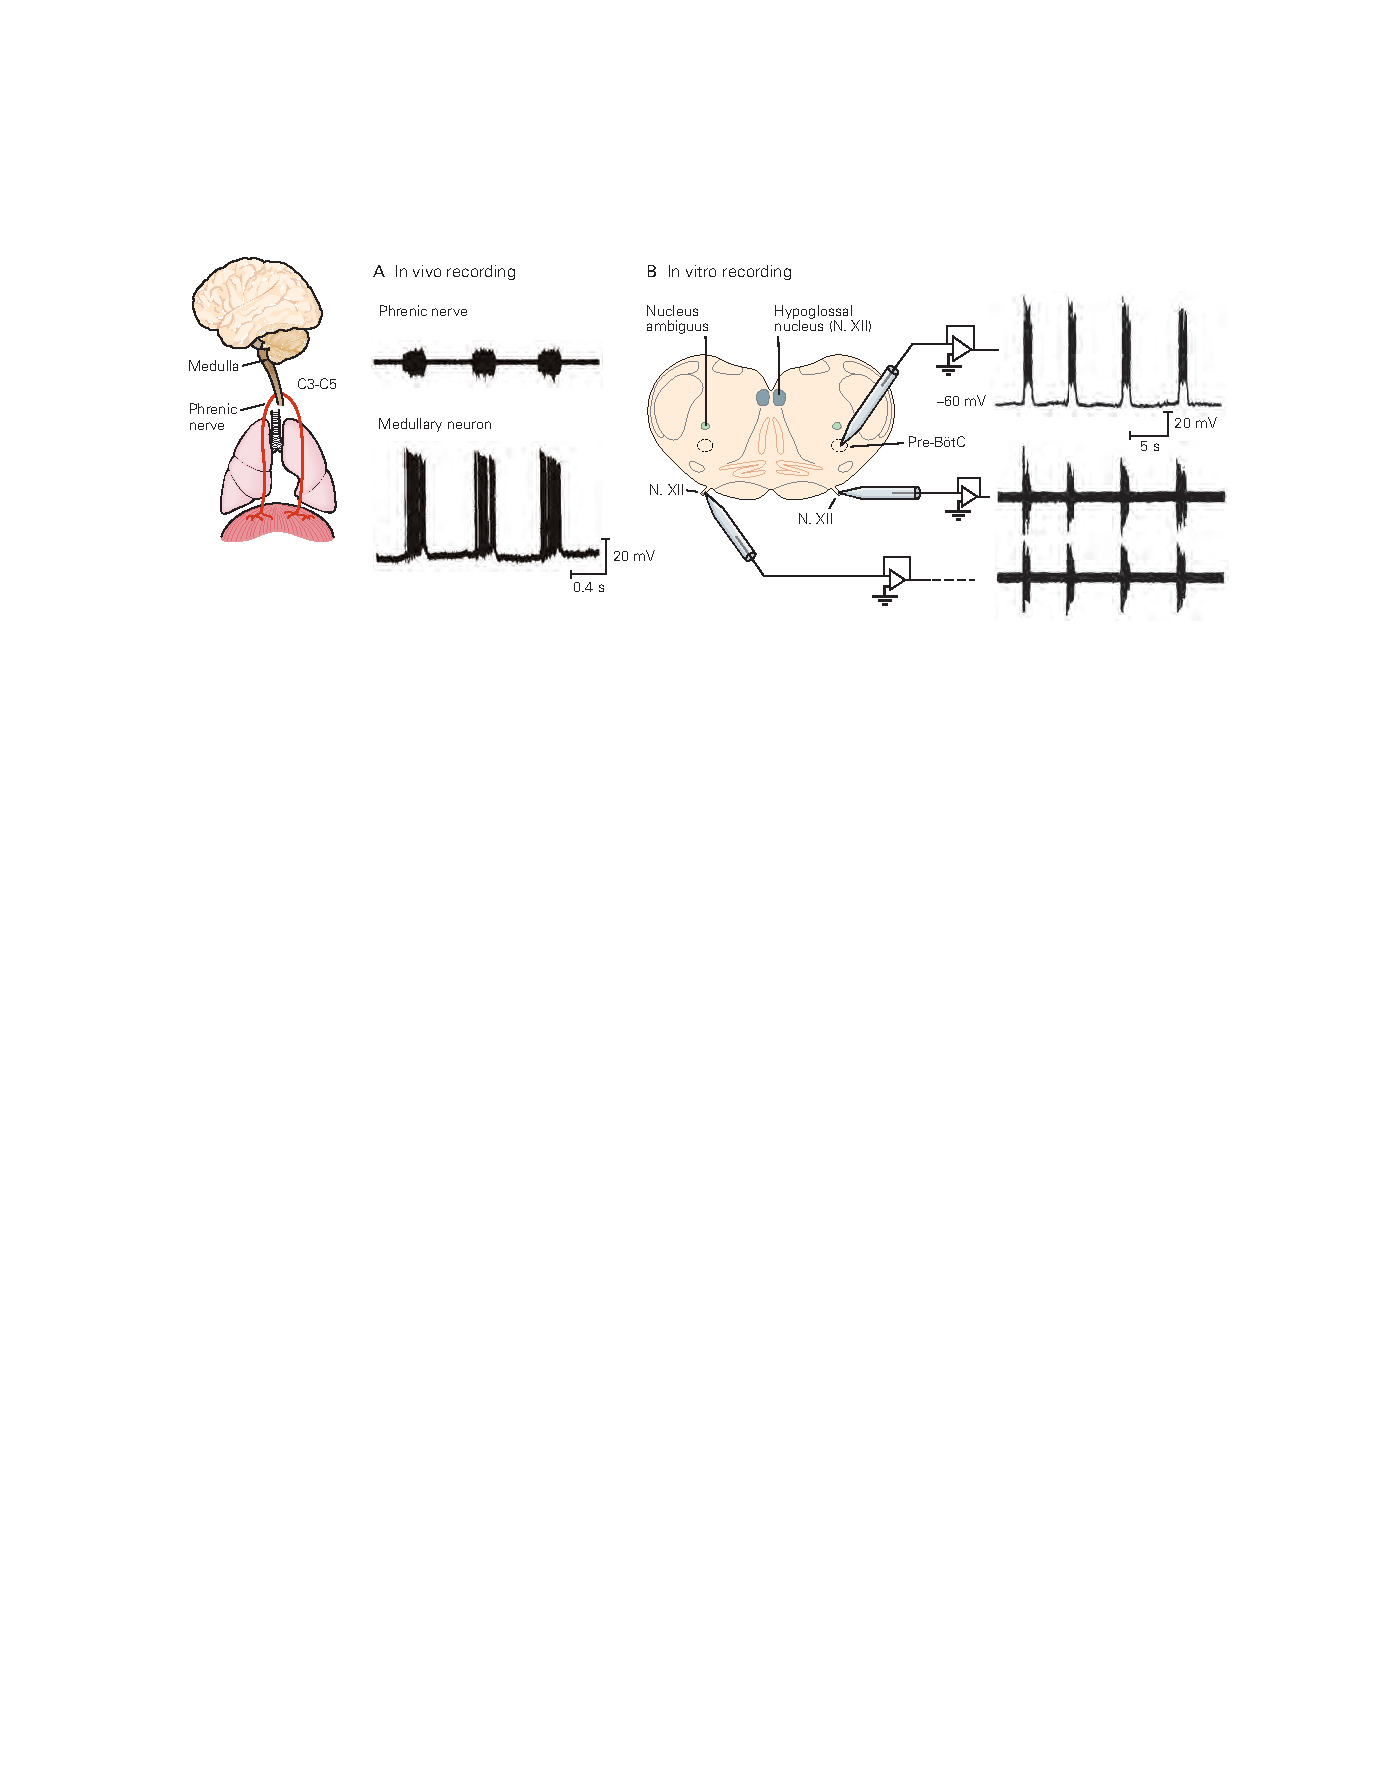
\includegraphics[width=1.0\linewidth]{chap40/fig_40_8}
	\caption{在延髓内产生有节奏的呼吸。 
		\textbf{A.} 豚鼠膈运动神经的节律活动导致横膈膜收缩。
		膈神经的放电被锁相到髓质中神经元的放电爆发。
		显示了细胞内记录的单个髓质神经元的活动\cite{richerson1987maintenance}。
		\textbf{B.} 类似的节律性放电可以从副呼吸神经(例如舌下神经 (XII))在体外记录到。
		支持这种节律所需的最小组织是延髓头端水平约 0.5 毫米厚的切片。
		\textit{前包钦格复合体}中的神经元靠近与运动节律锁相的疑核火爆\cite{smith1991pre}。}
	\label{fig:40_8}
\end{figure}


背侧呼吸群位于孤束核腹外侧部的两侧和周围。
该组中的神经元接受呼吸感觉输入,包括来自肺部牵张感受器和外周化学感受器的传入,并参与诸如限制高容量肺膨胀(\textit{黑-伯反射})和对低氧的通气反应等反射作用。
腹侧呼吸组是疑核内和周围的一列神经元,协调呼吸运动输出。
这些神经元中的一些是带有轴突的运动神经元,它们通过迷走神经离开大脑并支配呼吸的辅助肌肉或支配膈运动核的运动前神经元,而其他神经元形成模式发生器,\textit{前包钦格复合体},产生呼吸节律。


\textit{前包钦格复合体}的内在节律性是如此有弹性,以至于即使在来自延髓头端的横向脑切片中,\textit{前包钦格复合体}中的神经元也能够独立产生可以在舌下神经根中记录的呼吸节律 (XII) 从切片的腹面出现的神经(图~\ref{fig:40_8}B)。
完整动物体内这种细胞群的急性破坏会导致无法维持正常的呼吸节律。


呼吸模式发生器最重要的输入来自感知氧气和二氧化碳的化学感受器。
在正常情况下,通风主要受 CO$_2$ 水平而非 O$_2$ 水平的调节(图~\ref{fig:40_9}A)。
然而,如果 O$_2$ 变得足够低,例如在高海拔地区或患有肺部疾病的人,呼吸也会受到强烈刺激。
颈动脉和主动脉体中的外周化学感受器通常主要对血氧减少做出反应,但在缺氧期间,它们也会对升高的 CO$_2$ 水平(高碳酸血症)更加敏感。
来自颈动脉窦神经的传入纤维在舌咽神经中传播并激活背侧呼吸组中的神经元。


\begin{figure}[htbp]
	\centering
	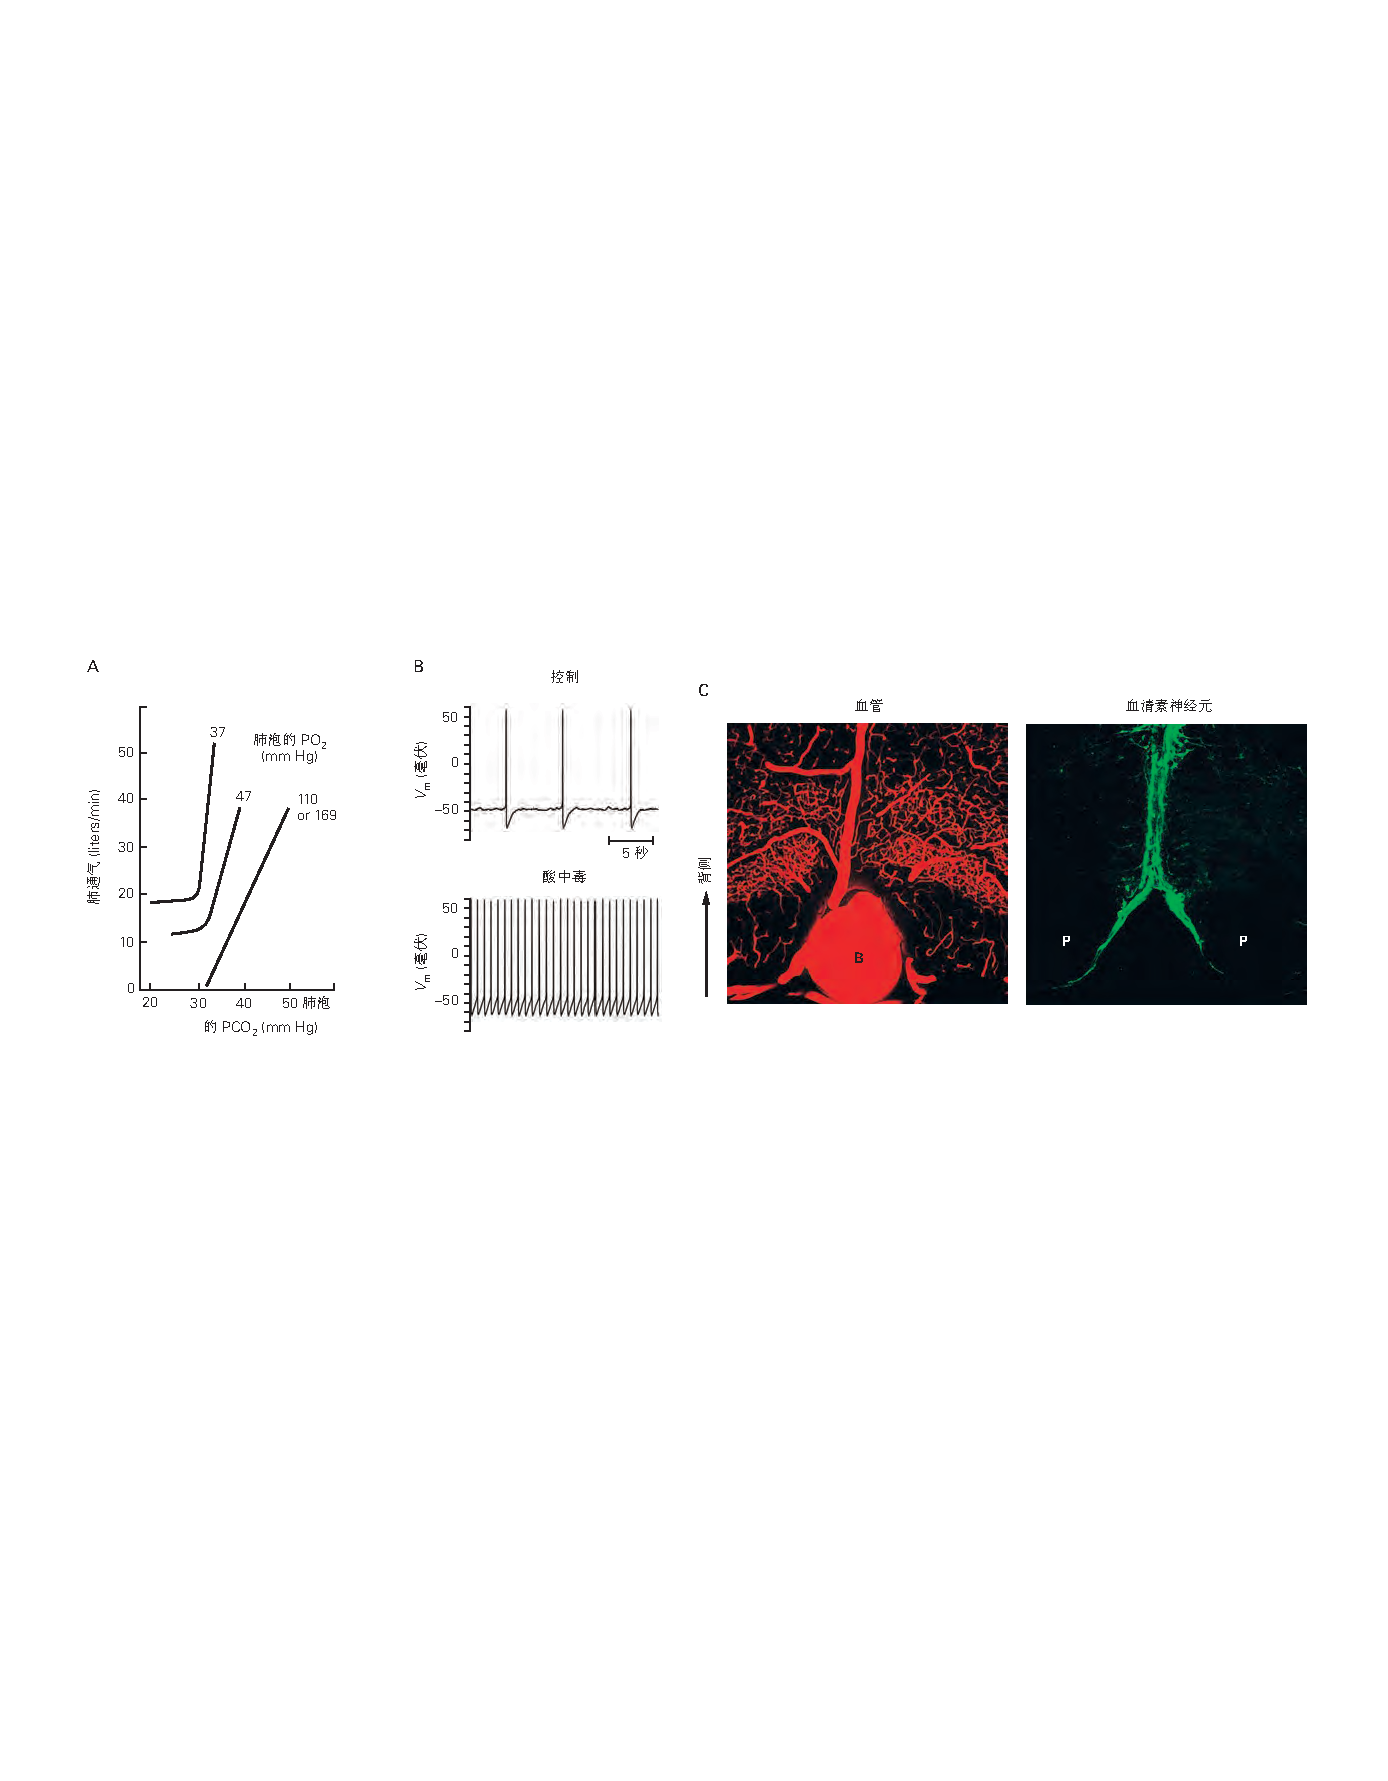
\includegraphics[width=1.0\linewidth]{chap40/fig_40_9}
	\caption{呼吸运动输出受血液中二氧化碳的调节。
		\textbf{A.} 人类的肺通气量(由呼吸频率和深度决定)在正常氧分压 (PO$_2$) (>100 mm Hg) 水平下严重依赖于\textit{二氧化碳分压}。
		当PO$_2$降至非常低的值(<50 毫米汞柱)时,呼吸会受到直接刺激,并且对\textit{二氧化碳分压}的增加也变得更加敏感(此处视为肺泡PO$_2$曲线斜率增加 37 和 47 毫米汞柱)。
		\textbf{B.} 髓质中的中央化学感受器控制通气运动输出以维持正常的血液 CO$_2$。
		当升高的\textit{二氧化碳分压}导致 pH 值降低时,髓质中缝核内的血清素能神经元的放电率会增加。
		此处显示的记录来自大鼠中缝核神经元在两种不同 pH 水平(7.4,对照和 7.2,酸中毒)下的体外记录\cite{wang2002quantification}。
		\textbf{C.} 5-羟色胺能神经元与腹侧延髓中的大动脉密切相关,在那里它们可以监测\textit{二氧化碳分压}的局部变化。
		大鼠髓质同一横截面的两张图像显示了动脉系统注射红色荧光染料后的血管(左)和色氨酸羟化酶(合成血清素的酶)的绿色抗体染色(右)。
		基底动脉 (B) 位于锥体束 (P) 之间的髓质腹侧表面\cite{bradley2002chemosensitive}。}
	\label{fig:40_9}
\end{figure}


对高碳酸血症的反应主要由脑干中的中枢化学感受器驱动,这些感受器感知伴随的 pH 值下降。
对此最敏感的区域是沿着锥体束外侧的髓质腹面。
该区域至少包含两组对升高的二氧化碳有反应的神经元。
靠近面部运动核的头端腹外侧延髓后梯形核中的谷氨酸能神经元对 CO$_2$ 水平高度敏感。
由于发育所需的 phox2b 转录因子发生突变,这些神经元的缺失会导致先天性中枢性通气不足综合征,即无法充分呼吸,尤其是在睡眠期间。
此外,髓质头端腹外侧的 5-羟色胺能神经元,如后梯形神经元,位于穿透动脉中,对酸中毒敏感(图 40-9B、C)。
这些神经元的基因缺失会降低对高碳酸血症的通气反应,尤其是在睡眠期间。
最近的研究表明,5-羟色胺 \textit{5-羟基色氨酸}A 激动剂可以恢复对 CO$_2$ 的唤醒反应,表明 5-羟色胺能神经元发挥调节作用,增加高碳酸血症期间 CO$_2$ 反射的敏感性,这在睡眠期间可能尤为重要。


健康人的呼吸系统产生的运动模式非常稳定,但多种疾病可以改变这些模式。
最常见和最容易识别的模式之一是陈-斯托克斯呼吸,其特征是通气逐渐增加然后减少的重复循环,与呼吸停止(呼吸暂停)交替出现。
例如,在先天性中枢通气不足综合征中可以看到这种周期性呼吸,其中中枢神经元对升高的二氧化碳不够敏感,尤其是在睡眠期间。 当他们开始做出反应时,二氧化碳水平可能已经很高了。
这会导致换气过度,从而将二氧化碳水平降低到需要呼吸的阈值以下。
结果是一段时间的呼吸暂停,直到二氧化碳水平再次变得相当高(图~\ref{fig:40_10})。


\begin{figure}[htbp]
	\centering
	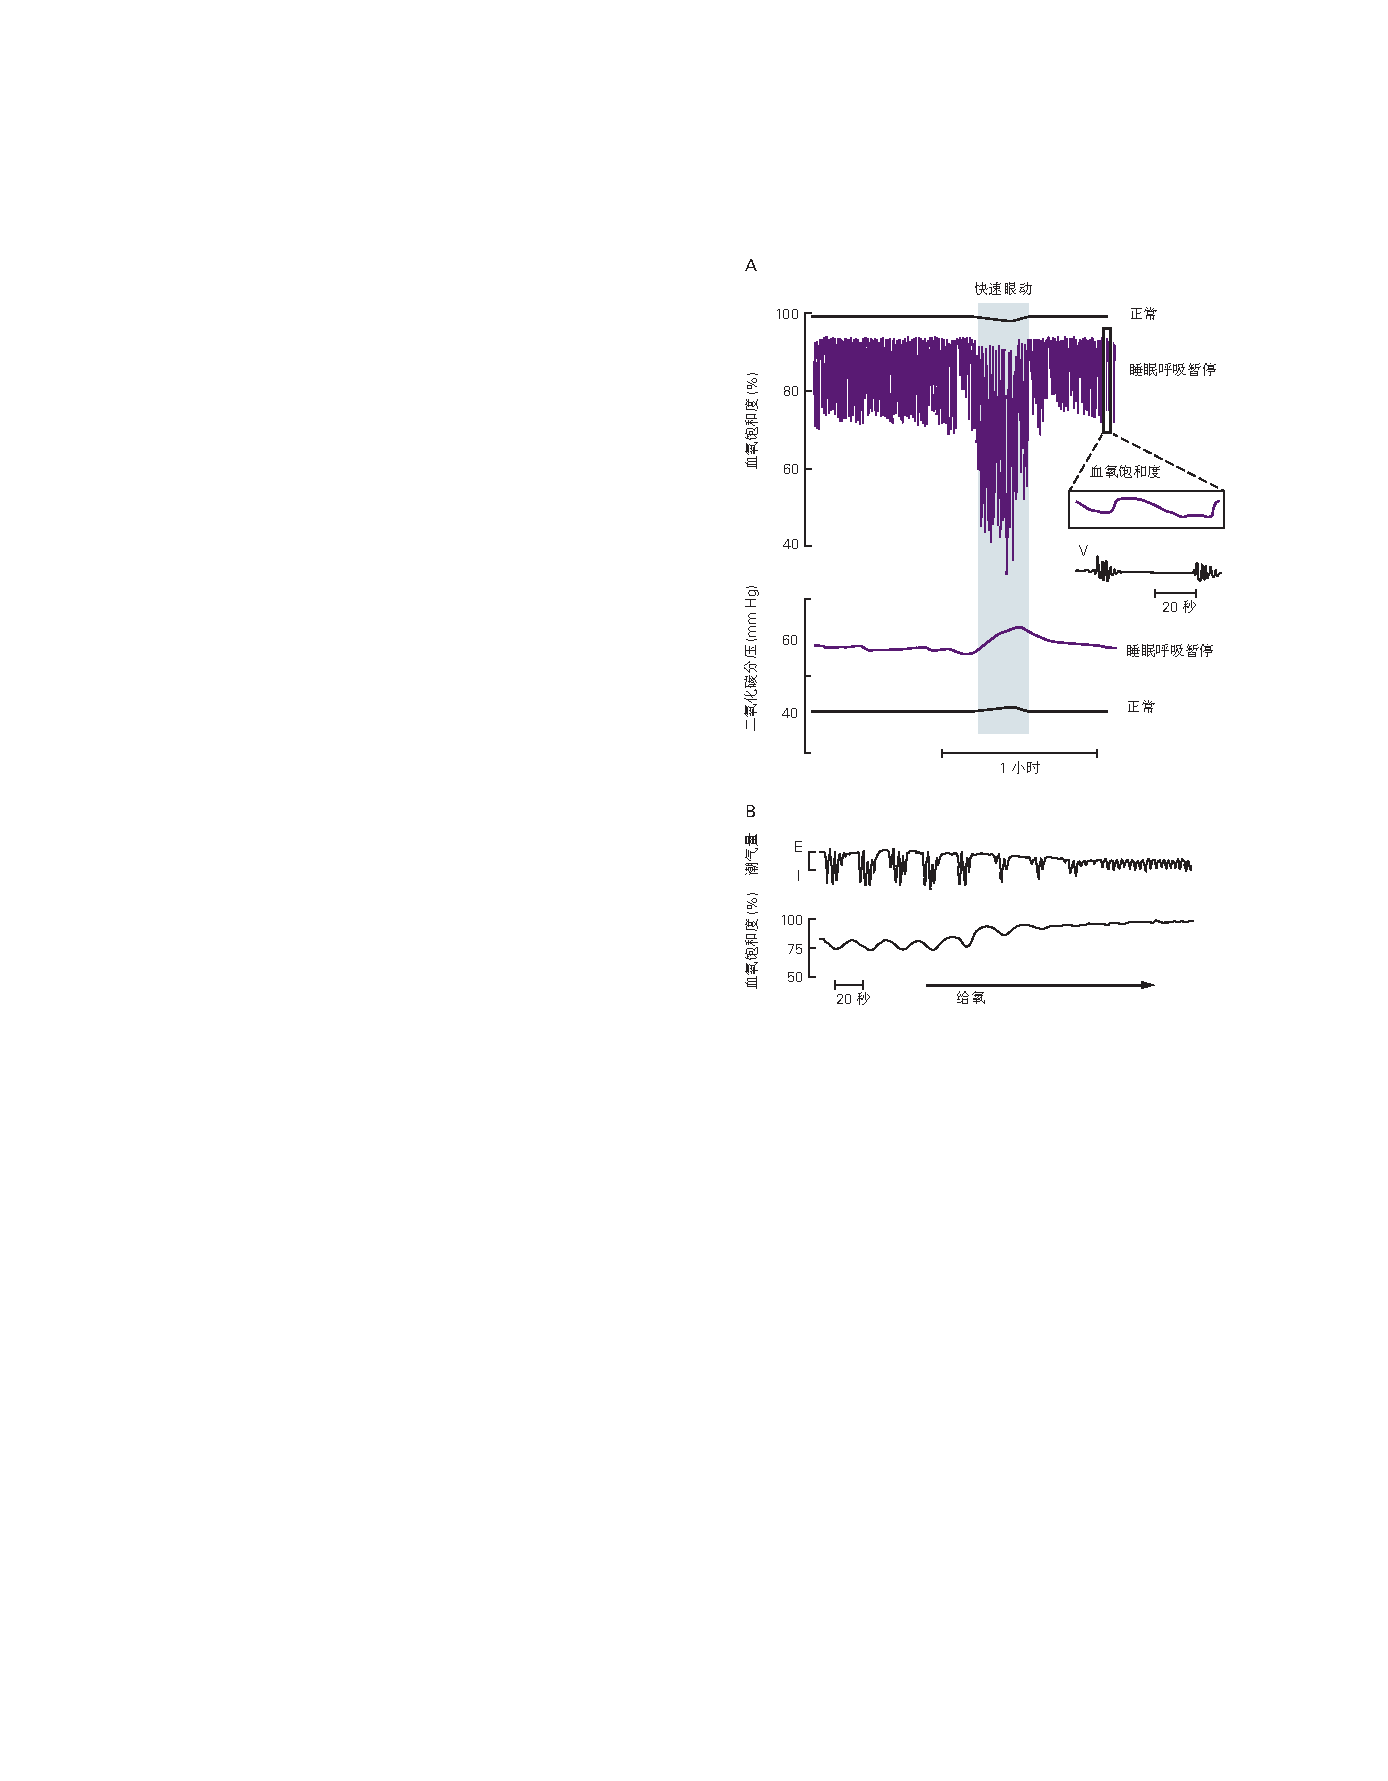
\includegraphics[width=0.7\linewidth]{chap40/fig_40_10}
	\caption{呼吸运动模式在睡眠期间会变得不稳定。
		\textbf{A.} 睡眠呼吸暂停(呼吸停止)是一种常见问题,但往往未被发现。
		此处的记录显示健康人和阻塞性睡眠呼吸暂停患者睡眠期间的\textit{血氧饱和度}和\textit{二氧化碳分压}。
		在健康人中,在\textit{快速眼动}和非快速眼动睡眠期间,\textit{血氧饱和度}保持在接近 100\%,\textit{二氧化碳分压}保持在接近 40 mm Hg。
		在患有睡眠呼吸暂停的患者中,睡眠期间肌张力降低(肌张力减退)会导致上呼吸道塌陷,从而导致阻塞和呼吸暂停。
		以大约每分钟一次的速度重复呼吸暂停会导致患者的\textit{血氧饱和度}反复急剧下降。
		(插图显示了大约 80 秒的扩展时间段。
		通气 [V] 在\textit{血氧饱和度}的最低点开始,并在血氧增加时再次停止。)
		在\textit{非快速眼动}睡眠期间,患者的 \textit{二氧化碳分压}增加到接近 60 mm 汞。 
		在\textit{快速眼动}睡眠期间,\textit{血氧饱和度}和\textit{二氧化碳分压}变得更加异常,因为恶化的气道肌张力减退会导致更大的阻塞。
		许多患有睡眠呼吸暂停症的人会因为呼吸暂停症而在夜间反复醒来,但觉醒时间太短,以至于他们没有意识到自己的睡眠被打断了\cite{grunstein1990neural}。 
		B. 大多数正常人的呼吸在高海拔地区的睡眠中变得不稳定。
		上面的曲线显示了健康人的潮式呼吸模式示例,在到达 17,700 英尺高度后的第一个晚上,空气中的低氧分压使血液中的\textit{血氧饱和度}降低到大约 75\% 80\%。
		通气渐强和渐弱的重复周期被呼吸暂停周期分开。
		给予补充氧气会导致快速恢复正常的呼吸模式。
		大多数人适应海拔高度后,这种异常模式就会消失\cite{lahiri1984sleep}。}
	\label{fig:40_10}
\end{figure}


在患有心脏病或肺病的人身上可以看到类似的模式,这种模式会增加肺泡二氧化碳变化记录到髓质所需的时间。
\textit{潮式呼吸}经常发生在入睡时具有边缘心脏或呼吸储备的住院患者中,从而减少其他呼吸行为驱动。
虽然本身并不危险,但它可能表明存在严重的潜在心肺问题需要纠正。


呼吸模式发生器的其他输入来自调解特定行为的回路,因为呼吸必须与共享相同肌肉的许多运动动作协调。
为了完成这种协调,延髓中的呼吸神经元接收来自与发声、吞咽、嗅觉、呕吐和疼痛有关的神经元网络的输入。
例如,腹侧呼吸组与桥脑中臂旁复合体的一部分相连,称为脑桥呼吸组或呼吸中枢。
这些桥脑神经元协调呼吸与咀嚼和吞咽等行为。
它们会导致在完全吸气时屏住呼吸(称为呼吸暂停),这是进食和饮水时所必需的。
肺部的空气储备允许在必要时咳嗽,以排出可能进入呼吸道的任何食物或饮料。
三叉神经间区的其他神经元,在三叉神经运动核和主要感觉核之间,接收面部和上呼吸道感觉输入,并投射到延髓腹外侧以暂时停止呼吸,以防止意外吸入灰尘或水。


在说话、吃饭、唱歌、游泳或演奏管乐器时,自主运动通路可以接管呼吸控制。
下降的输入会导致运动开始时换气过度,因为预计氧气需求会增加。
事实上,这会导致运动期间血液中的二氧化碳持续下降——这与负反馈控制系统的预期相反。
来自边缘系统的其他下行输入会产生与疼痛或焦虑相关的过度换气,并且在某些人中,可能会导致自发性惊恐发作,其特征是过度换气和窒息感。
这些不同的下降输入允许呼吸与其他行为的有效整合,但它们最终必须屈服于维持血气稳态的需要,因为即使二氧化碳的少量增加也会导致严重的空气饥饿或呼吸困难。
因此,呼吸控制系统是脑干模式发生器的一个迷人例子,它必须足够稳定以确保生存,但又必须足够灵活以适应各种各样的行为。



\section{脑干中的单胺能神经元调节感觉、运动、自主神经和行为功能}

除了包含颅神经的主要感觉和运动核以及控制基本行为的反射和模式发生器机制之外,脑干还包含一组调节细胞群。
在 1970 年代一系列开创性的实验中,\textit{汉斯$\cdot$凯珀斯}使用新发现的轴突示踪剂逆行运输方法来识别脑干和间脑中有助于调节脊髓感觉和运动系统以及发送输入的细胞群,直接进入大脑皮层。
令人惊讶的是,这两组实验从神经轴的两端开始,确定了一个共同的基质,其作用是调节神经系统其他水平的回路,几乎就像是一个“自主系统” 脑。


这些细胞群与调节目标整体功能水平的前脑、脑干和脊髓有直接联系。
就像血清素能神经元设置二氧化碳反射的整体敏感性一样,脑干单胺能调节系统通过投射到脊髓和脑干中的感觉神经元(包括伤害感受系统)来调整各种感觉系统的整体反应性。
来自这些调节系统的下行投射也控制运动音调,这对于调整姿势和步态以及启动更精细的动作至关重要。
前脑的上行输入控制整体唤醒以及对奖励情况的反应。
虽然这些调节系统不足以自行完成运动、感觉或认知任务,但它们调整这些系统响应能力的能力对整体行为起着巨大的影响。



\subsection{许多调节系统使用单胺作为神经递质}

单胺能系统使用环状氨基酸酪氨酸、色氨酸和组氨酸的脱羧衍生物作为神经递质。
由于它们中的一些具有在暴露于甲醛时发出荧光的特性,因此它们是最先被识别和绘制的大脑中的一员。
在 1960 年代,\textit{达尔斯特伦}和\textit{富克塞}利用这一特性来识别脑干中的血清素能、去甲肾上腺素能和多巴胺能细胞群。
在 20 世纪 70 年代,随着能够绘制合成单胺的酶的免疫组织化学方法的发展,其他研究人员绘制了含有肾上腺素和组胺的神经元图谱。


一般来说,这些调节系统的细胞群与大脑中早期发现的细胞核不同。
单胺能细胞群不是形成紧凑的细胞体簇,而是倾向于形成纵向延伸穿过脑干和下丘脑的柱状物(见图~\ref{fig:40_6})。
因此,单胺系统用字母和数字指定,以避免与大脑的其他命名系统混淆(图~\ref{fig:40_11})。


\begin{figure}[htbp]
	\centering
	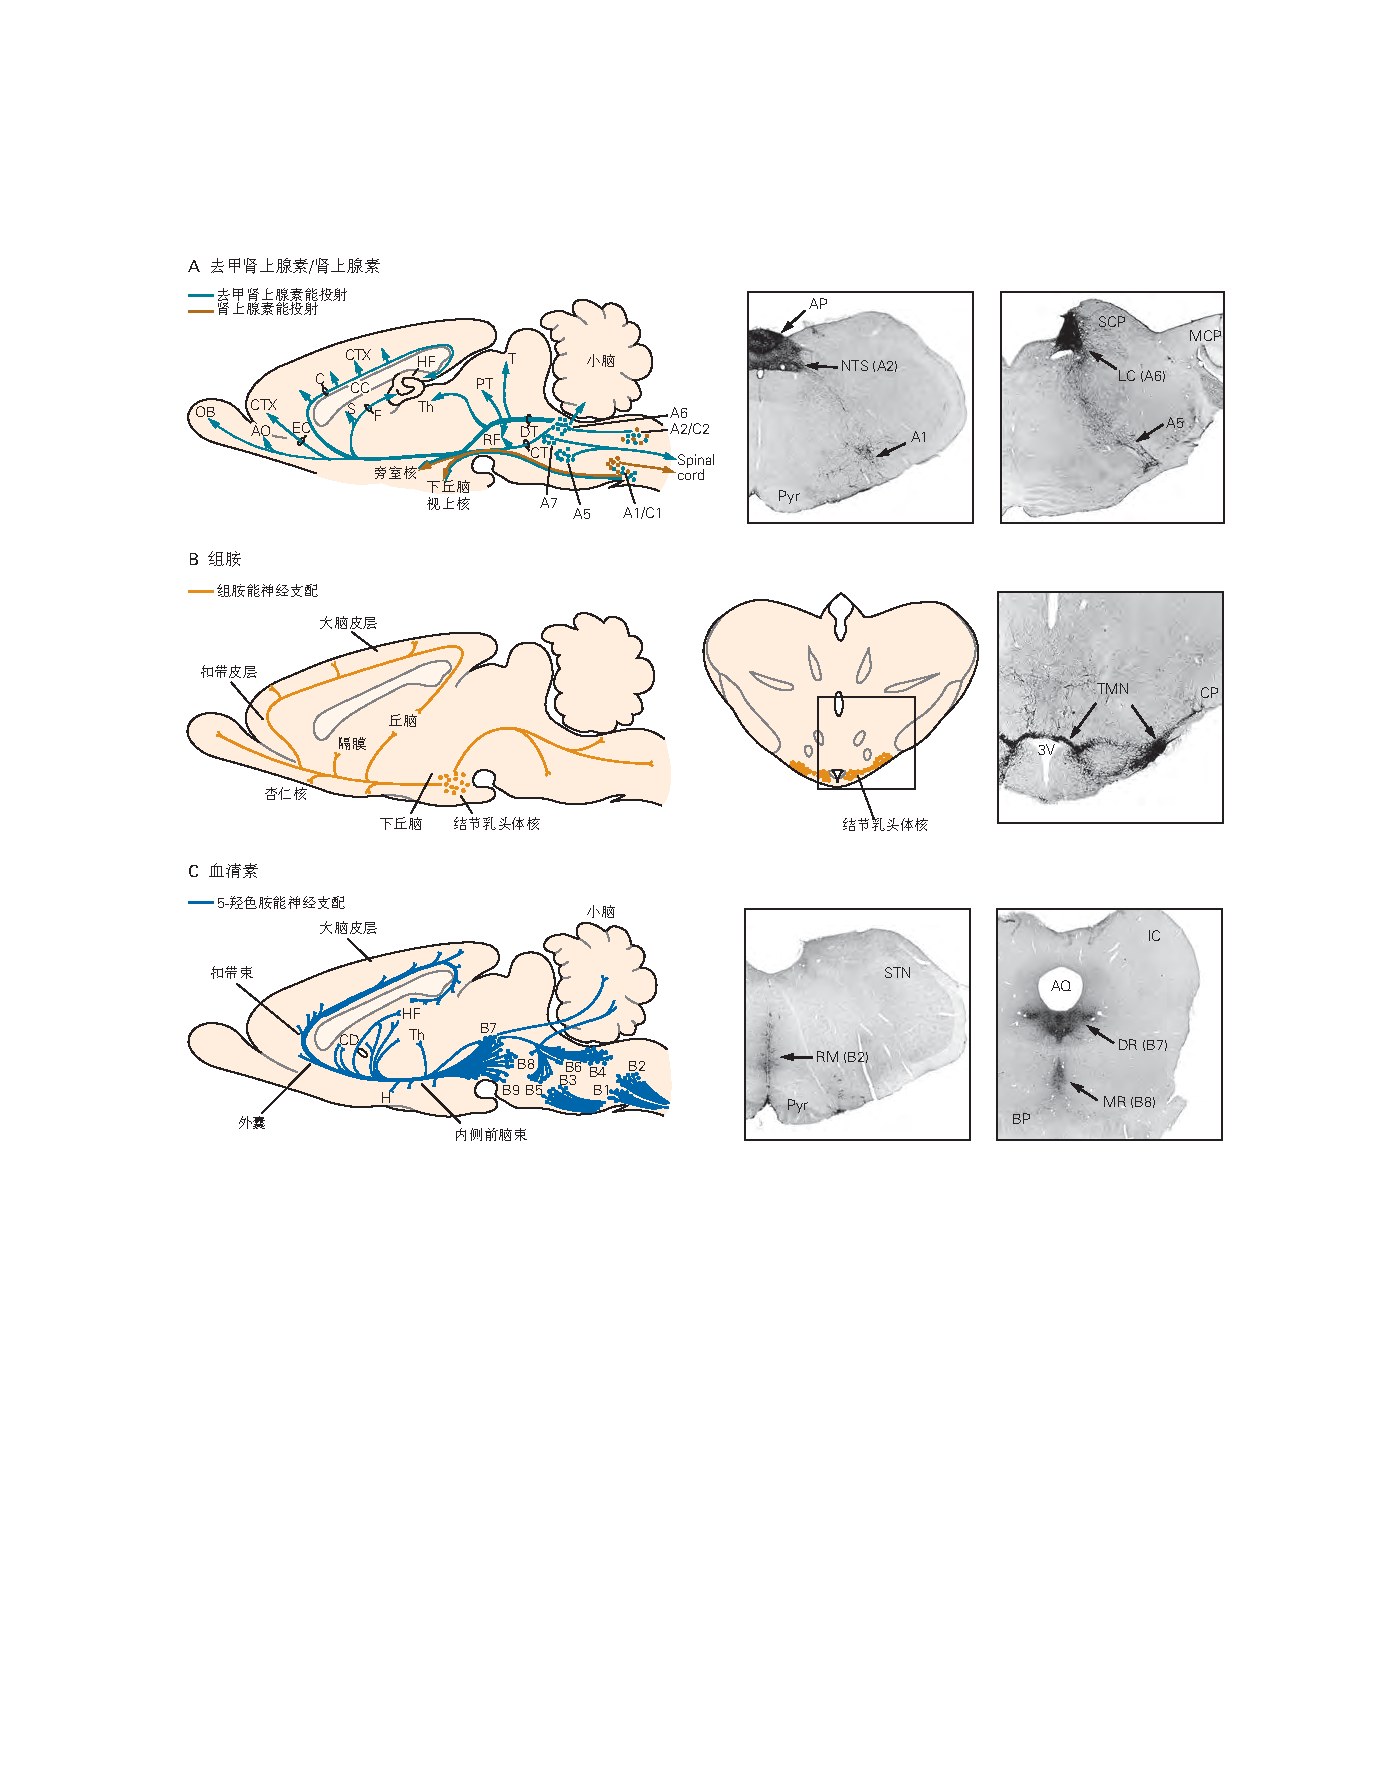
\includegraphics[width=1.0\linewidth]{chap40/fig_40_11}
	\caption{大鼠大脑中单胺能和胆碱能神经元的位置和投射。
		(缩写:3V,第三脑室;AC,前连合;AP,极后区;AQ,外侧裂导水管;ARC,弓状核;BM,Meynert 基底核;BP,桥脑;CD,尾状核;CP,大脑脚;DBh , 对角带的水平肢;DR,中缝背侧;FX,穹窿;IC,下丘;LC,蓝斑;LDT,背侧被盖核;MCP,小脑中脚;MGN,内侧膝状体核;MR,中缝; MS,内侧隔膜;MTT,乳头丘脑束;NTS,孤束核;OC,视交叉;PPT,脚桥被盖核;PUT,壳核;Pyr,锥体束;RM,大中缝;SC,上丘;SCP,小脑上 脚;SN,黑质;STN,脊髓三叉神经核;TMN,结节乳头核;VTA,腹侧被盖区。)
		\textbf{A.} 去甲肾上腺素能神经元(A 组)和肾上腺素能神经元(C 组)位于延髓和脑桥。
		延髓背侧的 A2 和 C2 组是孤束核的一部分。
		腹侧髓质中的 A1 和 C1 组位于疑核附近。
		两组都投射到下丘脑;
		一些 C1 神经元投射到脊髓中的交感神经节前神经元并控制心血管和内分泌功能。
		脑桥中的 A5、A6(蓝斑)和 A7 细胞群投射到脊髓并调节自主神经反射和痛觉。
		蓝斑也突出到前脑,在唤醒和注意力方面起着重要作用。
		\textbf{B.} 所有组胺能神经元都位于下丘脑后外侧,大部分位于结节乳头核内。
		这些神经元几乎投射到神经轴的每个部分,并在唤醒中发挥重要作用。
		\textbf{C.} 血清素能神经元(B 组)存在于延髓、脑桥和中脑内,大部分位于中缝核的中线附近。
		髓质内的那些(对应于大中缝、暗中缝和苍白中缝的 B1-B4 组)投射到整个髓质和脊髓并调节传入疼痛信号、体温调节、心血管控制和呼吸。
		脑桥和中脑内的那些(脑桥中缝、中缝和中缝背侧的 B5-B9 组)投射到整个前脑并有助于觉醒、情绪和认知。}
	\label{fig:40_11}
\end{figure}


\textit{达尔斯特伦}和\textit{富克塞}鉴定的第一个细胞群被简单地按字母顺序识别为“A”细胞群,然后从尾端到头端按顺序编号。
后来确定 A1-A7 细胞群产生去甲肾上腺素,A8-A14 细胞群产生多巴胺。
A1、A3 和 A5 名称适用于位于延髓和脑桥被盖腹外侧角的神经元(A3 组非常小,不再使用该术语),而 A2、A4、A6 和 A7 名称 被应用于位于更靠背的细胞群,类似于脑干中的运动神经元列(图~\ref{fig:40_11}A)。
A1 和 A2 组分别位于疑核和孤束核的神经元之间,主要与自主神经功能有关。
它们一起调节调节自主神经系统的下丘脑和脑干系统。
去甲肾上腺素能 A4-A7 细胞群对从大脑皮层到脊髓的感觉和运动系统具有广泛的影响,并提供重要的觉醒和觉醒调节。


多巴胺能系统(图~\ref{fig:40_11}E)包括位于中脑黑质附近的 A8-A10 细胞群,它调节运动系统以及奖励和动机的前脑机制。
背侧下丘脑中的 A11 和 A13 多巴胺能神经元为脑干和脊髓中的感觉、运动和自主神经系统提供输入。
A12、A14 和 A15 神经元具有神经内分泌作用,包括释放多巴胺作为催乳素分泌的垂体释放抑制激素。
A16 细胞群调节嗅觉输入,视网膜中的 A17 神经元调节视觉。


发现荧光颜色略有不同的 B 细胞群会产生血清素。
它们与脑桥和延髓中的中线中缝细胞群有关(图~\ref{fig:40_11}C)。
髓质中的 B1-B4 细胞群主要提供脑干和脊髓中感觉、运动和自主神经元的下行调节。
脑桥中的 B5-B7 神经元主要提供丘脑、下丘脑和大脑皮层的血清素能神经支配。
血清素在调节这些靶标中的功能可能非常复杂,难以破译,主要是因为至少有 14 种不同的血清素受体,并且不同的受体可以由靶标区域中的不同细胞类型表达。


在命名 A 和 B 细胞群几年后,免疫组织化学研究表明,一些髓质神经元具有制造多巴胺和去甲肾上腺素的酶,但不发出荧光。
这些神经元被命名为 C1-C3 细胞群,被发现可以将这些其他儿茶酚胺转化为肾上腺素或肾上腺素。
它们与髓质中的 A1-A3 细胞群密切相关(图~\ref{fig:40_11}A)。


组胺能细胞群主要存在于结节乳头核和下丘脑后部的邻近区域(靠近乳头体),被命名为 E1-E5(图 ~\ref{fig:40_11}B)。
它们是整个大脑(从大脑皮层到脊髓)中组胺能作用的唯一来源,并参与各种唤醒反应。


虽然胆碱能神经元严格来说不是单胺能神经元,但它们中的一些也参与调节系统,这些被编号为 Ch1–Ch6(图 40–11D)。
该分类系统不包括神经系统中的许多其他胆碱能神经元,例如运动神经元或纹状体中间神经元,因此不再使用。
相反,科学家通过它们的位置来指代胆碱能神经元,例如,脑桥中的脚桥脑 (Ch6) 和背侧被盖 (Ch5) 神经元,它们从大脑皮层广泛投射到延髓,以及基底前脑 (Ch1–Ch4) 组,投射到大脑皮层、海马体和杏仁核。



\subsection{单胺能神经元具有许多细胞特性}

使用单胺类作为神经递质的神经元具有许多相似的电生理特性。
例如,当与大脑切片准备中的突触输入隔离时,大多数人会继续以高度规则的模式激发自发动作电位。
它们的动作电位之后通常会出现缓慢的膜去极化,从而导致下一个峰值(图~\ref{fig:40_12})。
单胺能神经元的自发规律放电模式受固有起搏器电流的调节(第~\ref{chap:chap10}~章)。
体内补品激发对于确保单胺持续递送至靶标可能很重要。
例如,基底神经节依赖于持续暴露于来自黑质神经元的多巴胺以促进运动反应。


\begin{figure}[htbp]
	\centering
	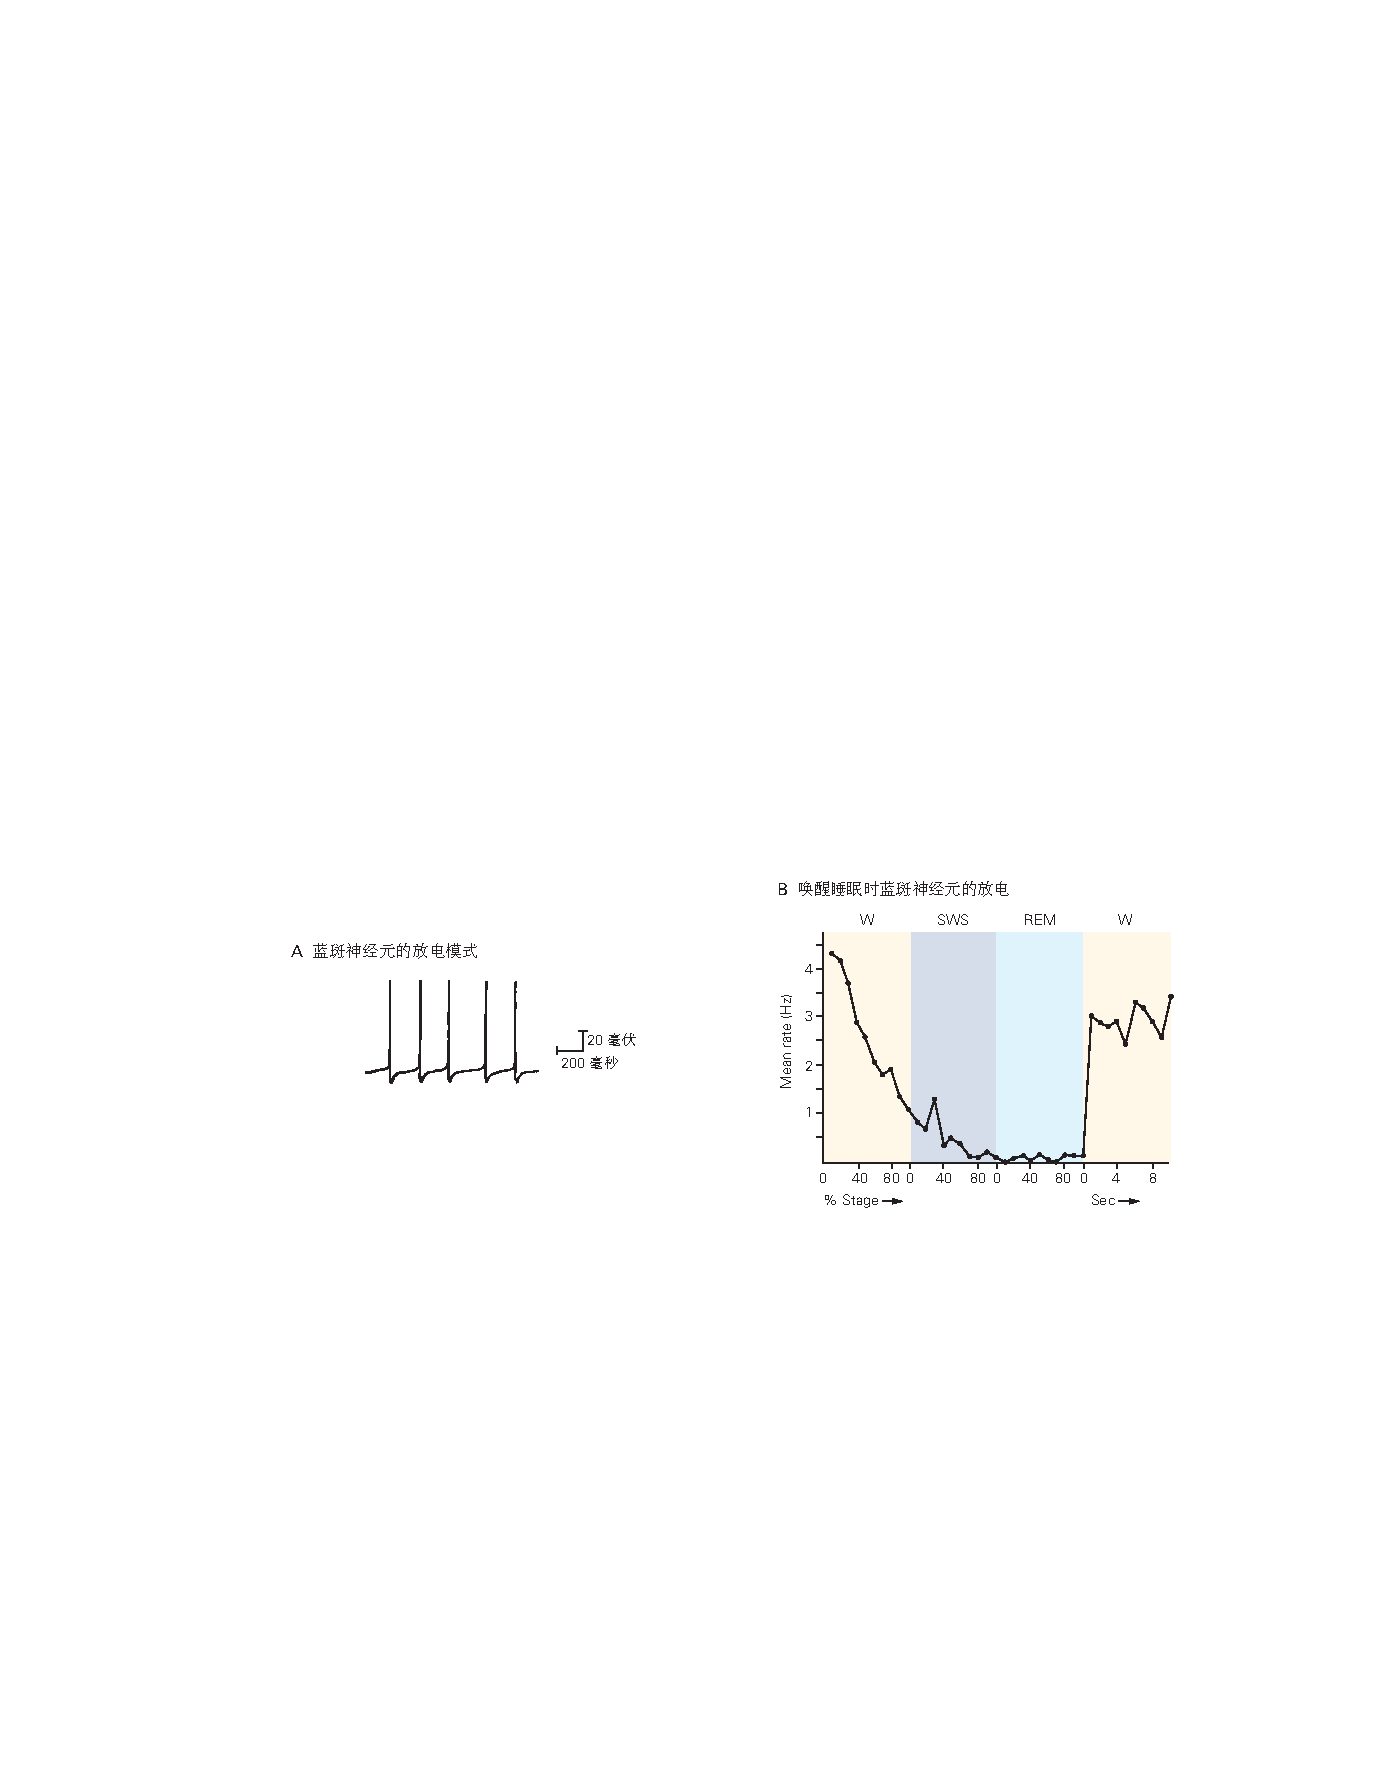
\includegraphics[width=0.85\linewidth]{chap40/fig_40_12}
	\caption{单胺能神经元在整个清醒-睡眠周期中具有相似的放电模式。
		\textbf{A.} 当单胺能神经元与突触输入隔离时,它们会以固定速率自发放电。
		这段录音来自蓝斑中的去甲肾上腺素能神经元。
		动作电位之后是特征性的后超极化,然后是下一个尖峰的缓慢去极化,产生类似起搏器的活动(第~\ref{chap:chap10}~章)。
		血清素能和组胺能神经元表现出相似的自发活动。
		\textbf{B.} 所有三种单胺能细胞类型在整个清醒-睡眠周期中都显示出相似的放电模式。
		该图显示大鼠的蓝斑神经元在动物清醒时放电最快,随着清醒减弱和\textit{慢波睡眠}减慢,并且在睡觉\textit{快速眼动}期间几乎完全停止放电\cite{aston1981activity}。}
	\label{fig:40_12}
\end{figure}


单胺能神经元的特性与其在大脑功能中独特而广泛的调节作用相适应。
事实上,一些单胺能细胞的轴突末端甚至不形成传统的突触连接,而是同时向许多目标扩散释放神经递质。
大多数单胺能神经传递是通过 G 蛋白偶联受体的促代谢突触作用发生的。
许多单胺能神经元共同释放神经肽,这些神经肽通过其他 G 蛋白偶联受体产生缓慢的作用。
因此,虽然一些单胺能突触作用涉及快速突触机制(第~\ref{chap:chap13}~章),但许多也涉及较慢的代谢和神经调节通路(第~\ref{chap:chap14}~章)。



\subsection{自主调节和呼吸由单胺能途径调节}

髓质头端腹外侧的肾上腺素能 C1 组神经元在维持静息血管张力以及调节各种行为所需的血管舒缩张力方面起着关键作用。
例如,直立姿势会抑制延髓头端腹外侧神经元的抑制,这些神经元直接支配交感神经节前血管运动神经元,从而增加血管运动张力以防止血压下降(压力感受器反射)。
脑桥中去甲肾上腺素能 A5 组的神经元会抑制交感神经节前神经元,并在降压反射中发挥作用(例如,对深度疼痛做出反应的血压下降)。


血清素调节许多不同的自主神经功能,包括胃肠蠕动、体温调节、心血管控制和呼吸。
电刺激中缝髓核内的血清素能神经元会增加心率和血压。
如前所述,髓质中的血清素能神经元也投射到调节呼吸的髓质和脊髓神经元。


血清素能神经元作为 CO$_2$ 受体的作用可以解释为什么血清素能系统缺陷与\textit{婴儿猝死综合症}有关(图 \ref{fig:40_13}A)。
\textit{婴儿猝死综合症}是西方世界新生儿死亡的主要原因,在美国每天有 6 名婴儿死亡。
一种广泛接受的理论认为,一些\textit{婴儿猝死综合症}病例是由于 CO$_2$ 化学感受、呼吸和觉醒缺陷所致。
在死于\textit{婴儿猝死综合症}的婴儿的中缝核中发现了相对较多数量的血清素能神经元,但这些神经元的形态不成熟,并且它们与相对较低的血清素水平和较低的血清素能受体密度有关。


\begin{figure}[htbp]
	\centering
	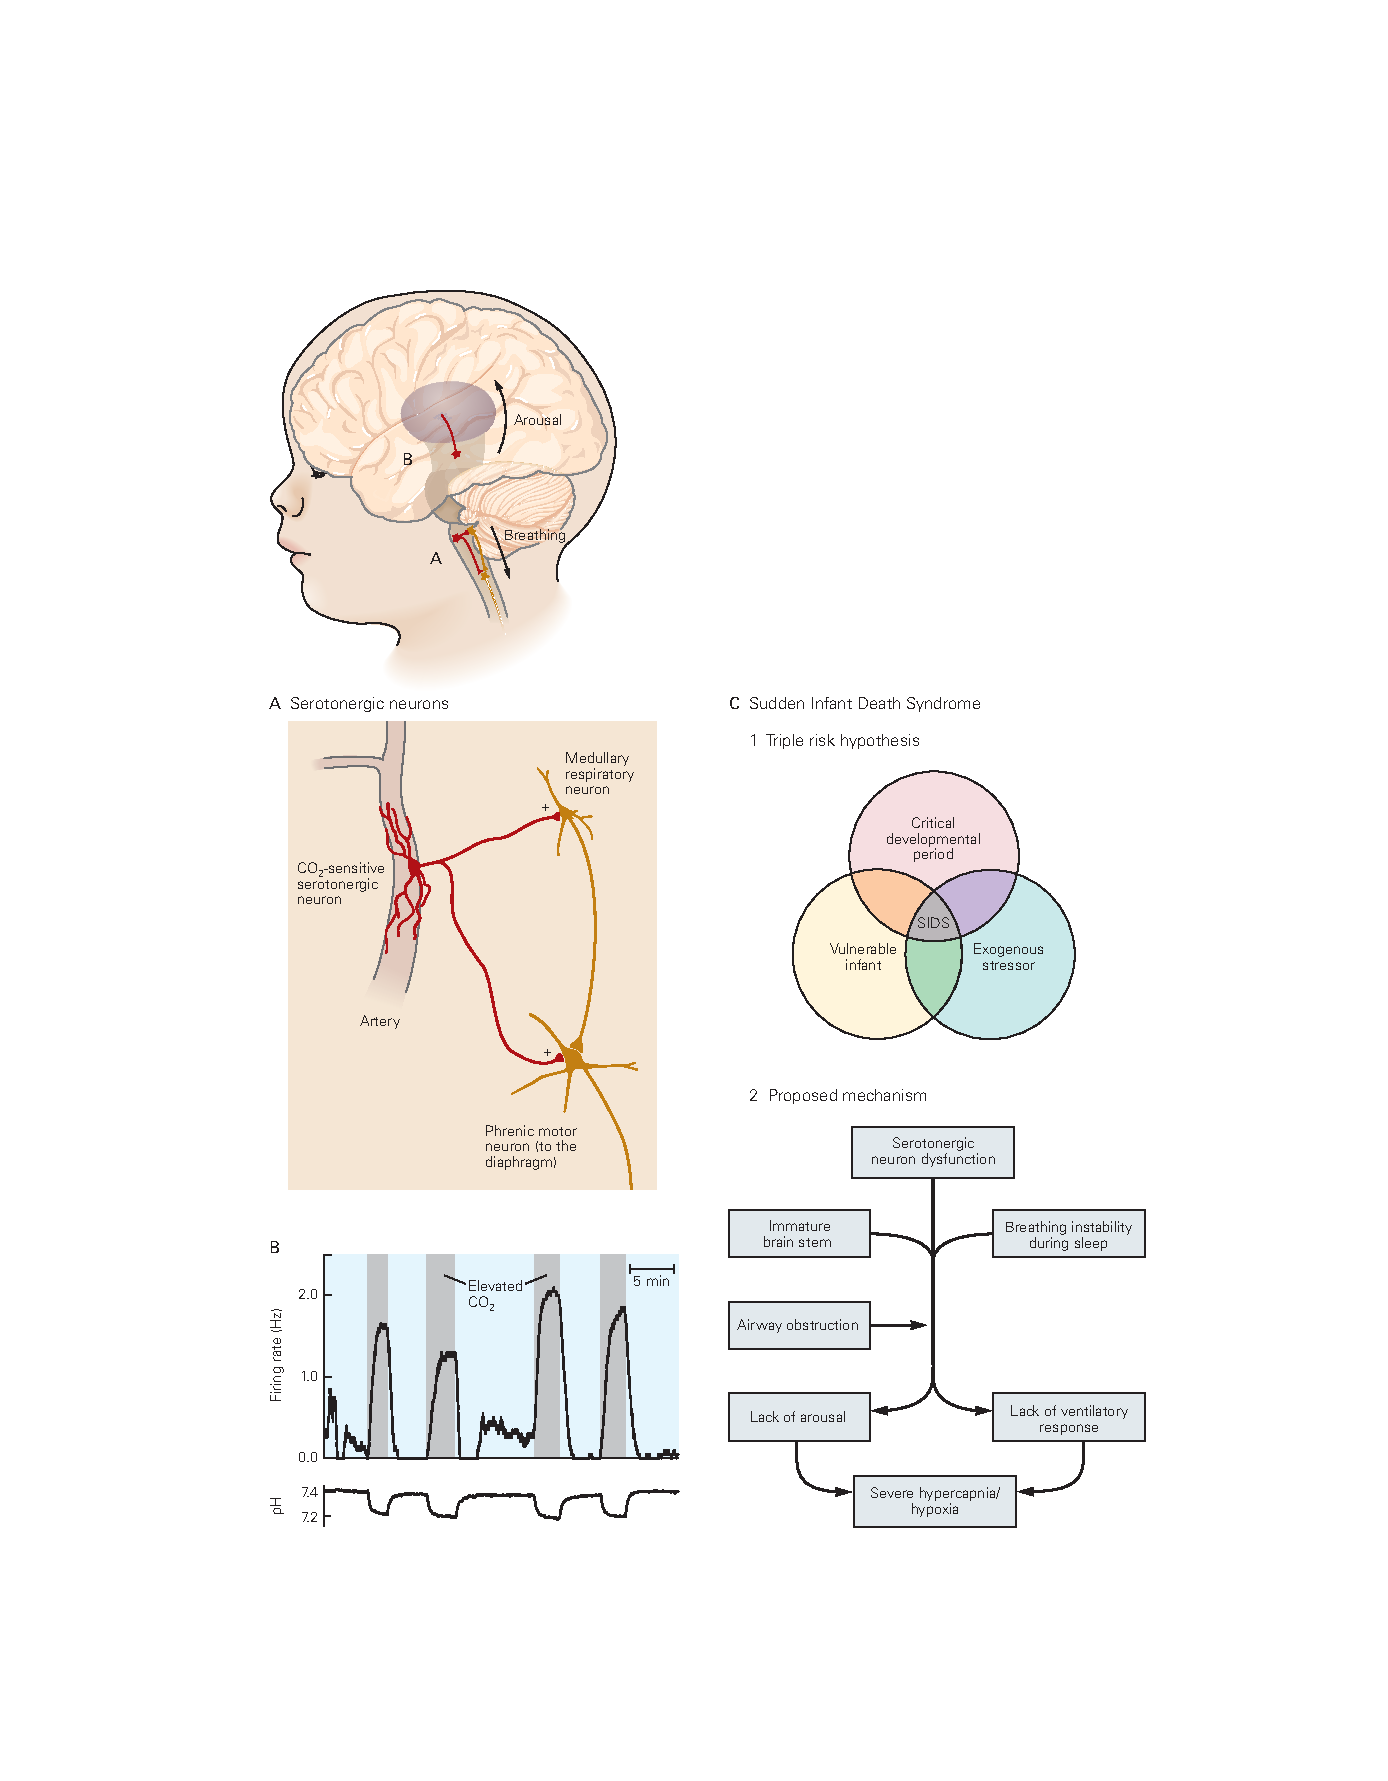
\includegraphics[width=1.0\linewidth]{chap40/fig_40_13}
	\caption{血清素能神经元在应对二氧化碳水平升高和婴儿猝死综合症方面发挥作用。
		\textbf{A.} 髓质中的血清素能神经元是中枢呼吸化学感受器,被认为可以刺激呼吸以响应动脉血\textit{二氧化碳分压}的增加。
		这些神经元的树突缠绕在大动脉周围,并受到\textit{二氧化碳分压}增加的刺激(见图~\ref{fig:40_9}C)。
		它们投射到并激发控制呼吸的髓质和脊髓中的运动神经元。
		\textbf{B.} 中脑中的血清素能神经元也是\textit{二氧化碳分压}传感器。
		这里显示的是来自中缝背核的血清素能神经元的放电率增加,以响应\textit{二氧化碳分压}的增加(通过外部 pH 值的降低来监测)。
		这种放电率的增加可能使来自臂旁核的上升觉醒通路敏感,臂旁核也接收来自其他 CO$_2$ 感觉通路的输入。
		当气道阻塞时,这种重要的反应可以防止睡眠时窒息\cite{richerson2004serotonergic}。
		\textbf{C.} \textit{婴儿猝死综合症}。 1. \textit{婴儿猝死综合症}的三重风险假说。
		当三种情况同时发生时,婴儿就有死于\textit{婴儿猝死综合症}的风险。
		首先,婴儿一定是易受伤害的,因为脑干有潜在的异常,例如遗传易感性或环境损害(例如,接触香烟烟雾)。 其次,婴儿必须处于发育阶段(通常为 2-6 个月大),此时可能难以改变姿势以避免窒息。
		第三,还必须有外源性压力源(例如,面朝下躺在枕头上)\cite{filiano1994perspective}。
		2. 拟议的\textit{婴儿猝死综合症}机制。
		异常的 5-羟色胺能神经元(例如,由于接触香烟烟雾)和出生后参与呼吸控制的神经元不成熟导致无法有效应对气道阻塞(例如,由于面朝下躺在婴儿床上)。
		然后婴儿不会醒来并转头或呼吸加快,这两种方法都可以解决问题。
		结果,血液中的氧合作用严重降低(缺氧),而血液中的二氧化碳升高(高碳酸血症)。}
	\label{fig:40_13}
\end{figure}


\textit{婴儿猝死综合症}的一个似是而非的神经生物学机制是,血清素能神经元的发育缺陷导致在睡眠期间气流受阻时检测 CO$_2$ 分压升高的能力降低,从而削弱正常的保护反应,包括唤醒和增加通气(图)\ref{fig:40_13}C)。
当床上用品阻塞呼吸道时,面朝下睡觉的婴儿将无法充分唤醒以改变姿势。
\textit{仰卧睡眠}运动鼓励父母让婴儿平躺睡觉,该运动已将\textit{婴儿猝死综合症}的发生率降低了 50\%。



\subsection{痛觉受单胺镇痛途径的调节}

虽然疼痛对于动物来说是减少伤害所必需的,但受伤后持续的疼痛可能是不适应的(例如,如果疼痛阻止了捕食者的有力逃脱)。
单胺能系统包括重要的下行投射到调节痛觉的脊髓背角(第~\ref{chap:chap20}~章)。


脊髓的去甲肾上腺素能输入源自脑桥细胞群 A5-A7,蓝斑 (A6) 为背角提供大部分输入。
同样,髓质中的 5-羟色胺能中缝核,尤其是中缝大核,投射到背角,在那里它们调节有害刺激信息的处理。
将 5-羟色胺直接应用于背角神经元会抑制它们对伤害性刺激的反应,而鞘内注射 5-羟色胺可减弱由伤害性刺激引起的爪子的防御性退缩。
此外,鞘内施用血清素受体拮抗剂可阻断刺激中缝核引起的疼痛抑制。


对血清素在疼痛处理中的作用的洞察已被用于治疗偏头痛。
特别是,已发现\textit{5-羟基色氨酸}1D受体的曲坦类激动剂具有治疗效果。
这一系列基于色胺的药物的可能作用机制之一包括抑制来自脑膜的疼痛传入,防止中枢神经元致敏。
阻断单胺再摄取的药物,包括传统抗抑郁药和选择性血清素再摄取抑制剂,可有效限制慢性疼痛和偏头痛患者的疼痛。



\subsection{单胺能途径促进运动活动}

多巴胺能系统对于正常的运动性能至关重要。
一个巨大的投影从黑质致密部上升到纹状体,多巴胺能纤维作用于纹状体神经元受体以释放对运动反应的抑制(第~\ref{chap:chap38}~章)。


中脑多巴胺能神经元退化的帕金森病患者难以开始运动,也难以维持运动。
此类患者说话轻声细语,书写小字,步子小。 相反,促进纹状体多巴胺能传递的药物可能会导致意想不到的行为,从运动性抽动(小肌肉抽搐)到舞蹈病(大规模的肢体运动),再到复杂的认知行为(例如强迫性赌博或性活动) )。


正如\textit{斯滕$\cdot$格瑞那}首次展示的那样,血清素能神经元在调节运动程序中起着重要作用。
激活血清素受体的药物可诱发多动症、肌阵挛、震颤和强直,所有这些都是“血清素综合征”的一部分。
在重复性运动活动(例如进食、梳理毛发、运动和深呼吸)期间,观察到动物中缝神经元的放电增加。
相反,血清素能中缝和去甲肾上腺素能蓝斑神经元的放电实际上在\textit{快速眼动}睡眠期间发生的张力缺乏和缺乏运动期间停止。


脑桥中的去甲肾上腺素能细胞群也向运动细胞群发送广泛的投射。
这种调节输入作用于突触前 $\beta$- 和 $\alpha$1- 肾上腺素能受体,以促进运动神经元的兴奋性输入(第~\ref{chap:chap31}~章)。
这些影响的总和是促进运动神经元对刻板和重复行为(如有节奏的咀嚼、游泳或运动)的反应。
相反,压力期间增加的 $\beta$-肾上腺素能激活会加剧运动反应并产生震颤。
阻断 $\beta$-肾上腺素能受体的药物在临床上用于减少某些类型的震颤,音乐家通常在表演前服用药物以尽量减少颤抖。



\subsection{上升的单胺能投射调节前脑系统的动机和奖励}

前脑不断受到感官信息的轰炸,必须确定哪些刺激值得关注。
它还必须部分地根据经验(哪些行为在过去取得了有益的结果)来决定在许多可用行为中应该优先考虑哪些行为。
上升的单胺能系统在调节所有这些选择中起着关键作用。


如前所述,纹状体的多巴胺能输入可调节特定运动模式甚至认知模式表达的可能性。
低多巴胺水平会减少直接通路纹状体神经元(释放行为)的输出并增加间接通路纹状体神经元(抑制行为)的活动。
多巴胺也与基于奖励的学习有关。 奖励是动物会为之努力的对象或事件(第~\ref{chap:chap42}~章),并且有助于积极强化行为。
当意外给予奖励(如食物或果汁)时,多巴胺能神经元的活动会增加。
但是,在训练动物在条件刺激后期待奖励后,神经元的活动在条件刺激后立即增加,而不是在奖励后增加。
这种活动模式表明多巴胺能神经元提供奖励预测错误信号,这是强化学习中的一个重要因素。
多巴胺在学习中的重要性也得到了观察结果的支持,即多巴胺能系统的损伤会阻止基于奖励的学习。
对奖励和学习很重要的相同多巴胺能途径与许多滥用药物成瘾有关(第~\ref{chap:chap43}~章)。


蓝斑的去甲肾上腺素能神经元在注意力中起重要作用。
这些神经元在昏昏欲睡的猴子中具有较低的基线活动水平。
在警觉、细心的猴子中,细胞有两种放电模式。
在相位模式下,神经元的基线活动从低到中等,但就在猴子对它一直注意的刺激做出反应之前会出现爆发性放电。
这种活动模式被认为有助于选择性地注意即将启动行为的刺激。
相比之下,在强直模式下,活动的基线水平升高并且不会因响应外部刺激而改变。
当当前任务不再有益时,这种激发模式可能会促进寻找新的行为和注意力目标(图~\ref{fig:40_14})。


\begin{figure}[htbp]
	\centering
	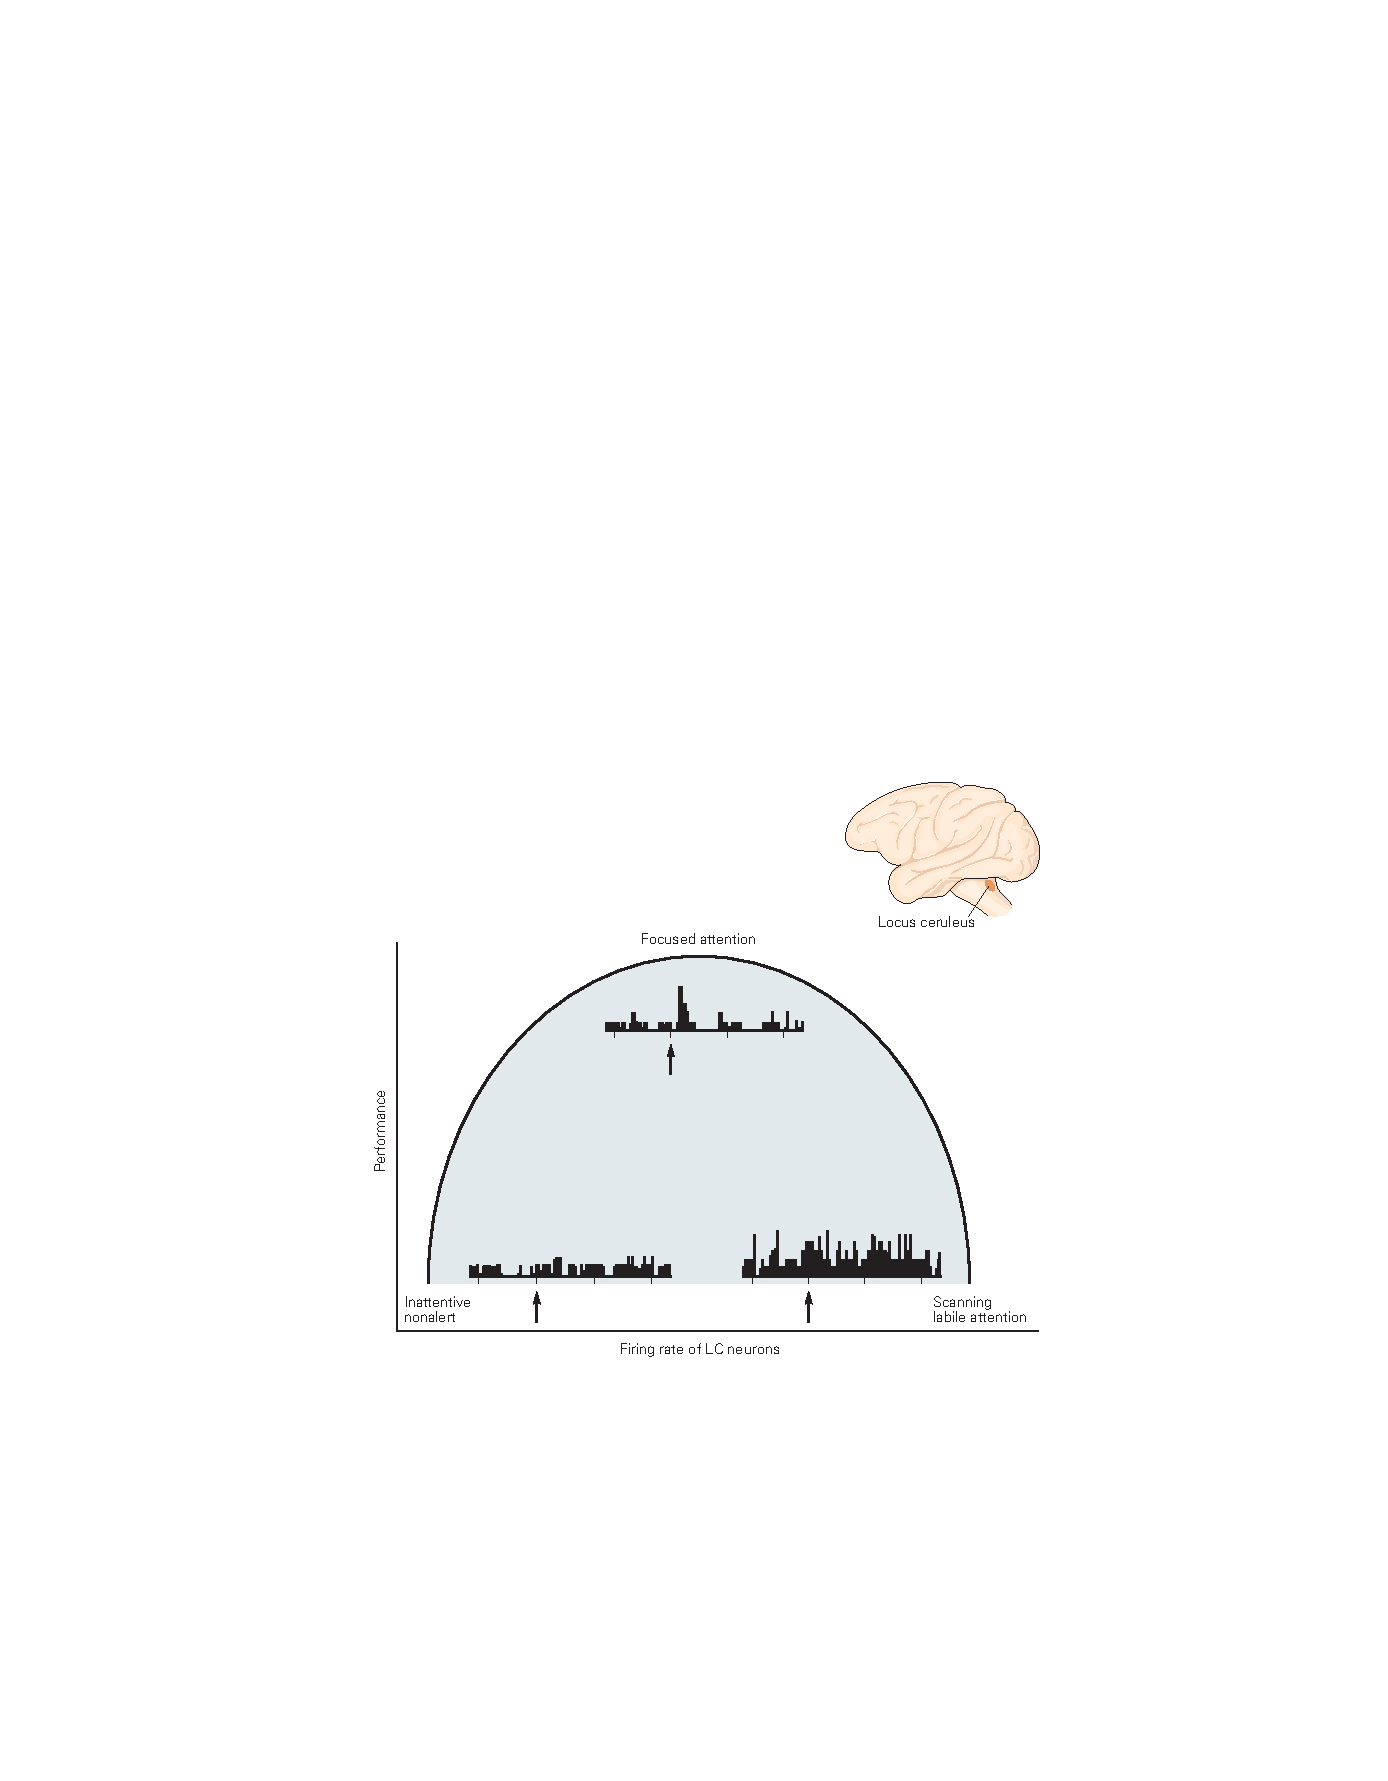
\includegraphics[width=0.75\linewidth]{chap40/fig_40_14}
	\caption{\textit{蓝斑}神经元表现出不同的活动模式,具有不同的注意力和任务表现水平。
		倒 U 型曲线显示了猴子在目标检测任务中的表现与蓝斑点活动水平之间的关系。
		直方图显示了\textit{蓝斑}神经元在不同级别的任务执行期间对目标呈现的反应。
		在低水平的\textit{蓝斑}活动下性能很差,因为动物不警觉。
		当基线活动适中并且阶段性激活遵循目标呈现时,性能最佳。
		当基线活动很高时,性能也会很差,因为较高的基线与专注于分配的任务不相容。
		补品模式(具有高基线活动)可能最适合需要行为灵活性而不是集中注意力的任务(或上下文)。
		如果是这样,\textit{蓝斑}可以调节专注和灵活行为之间的平衡\cite{aston1999role}。}
	\label{fig:40_14}
\end{figure}


许多单胺能神经元也参与调节整体觉醒(图~\ref{fig:40_15})。
去甲肾上腺素能蓝斑、5-羟色胺能背核和中缝核、多巴胺能 A10 神经元和组胺能结节乳头神经元支配丘脑、下丘脑、基底前脑和大脑皮层。
所有这些系统都具有在清醒期间发射最快、在慢波(或非快速眼动)睡眠期间减慢并在快速眼动睡眠期间逐渐停止的特性。


\begin{figure}[htbp]
	\centering
	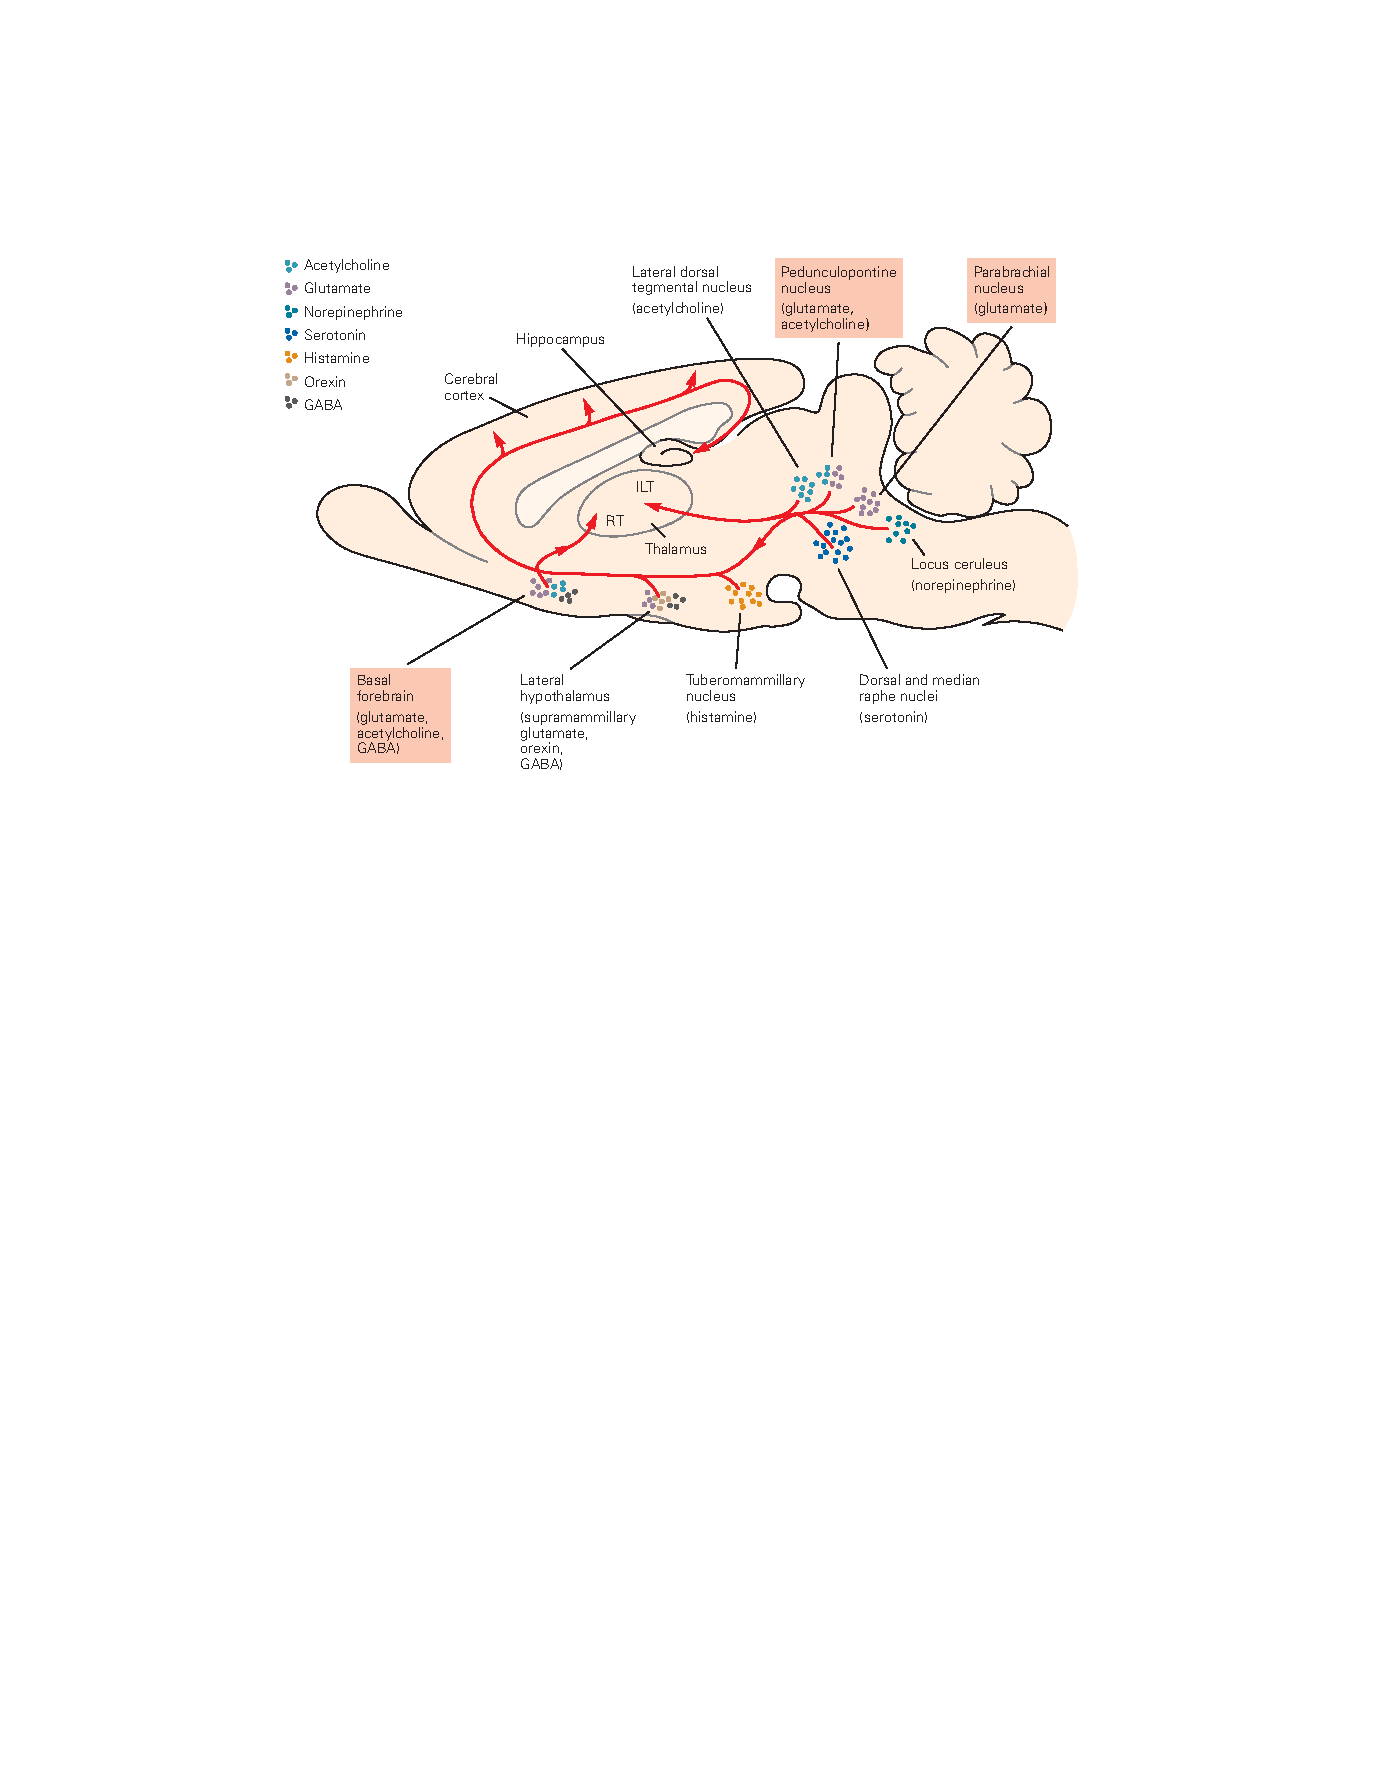
\includegraphics[width=0.9\linewidth]{chap40/fig_40_15}
	\caption{上行唤醒系统中的主要细胞群。
		使用神经递质去甲肾上腺素、血清素、多巴胺、组胺和乙酰胆碱的神经元具有广泛的前脑投射。
		尽管它们都通过调节各种大脑功能来促进觉醒,但消融这些细胞群中的任何一个对清醒状态影响不大,这表明它们都不是维持清醒状态所必需的。
		另一方面,臂旁核和桥足核中的谷氨酸能神经元或基底前脑(橙色框)中的 \textit{$\gamma$-氨基丁酸能}神经元、谷氨酸能神经元和胆碱能神经元的广泛损伤可导致深度和长时间的昏迷。
		因此,臂旁-足桥脑-基底前脑-皮层通路似乎是维持清醒状态所必需的唯一通路。}
	\label{fig:40_15}
\end{figure}


刺激蓝斑中的去甲肾上腺素能神经元或结节乳头核中的组胺能细胞会增加\textit{脑电图}觉醒,表明这些系统在皮层和行为觉醒中起重要作用。
然而,仅限于一个或什至一组单胺能细胞群的损伤不会导致严重的觉醒丧失,这表明各种细胞群可能在睡眠/觉醒调节中具有重叠和至少部分冗余的作用。
单胺能途径调节丘脑和大脑皮层突触后神经元的特定细胞特性,增强警觉性和与环境刺激的相互作用。



\subsection{单胺能和胆碱能神经元通过调节前脑神经元维持唤醒}

单胺能神经元和胆碱能神经元通过直接和间接激活皮层神经元来诱导觉醒。
他们通过调节激活大脑皮层的脑干、下丘脑、基底前脑和丘脑中神经元的活动来实现这一点。


去甲肾上腺素能神经元和血清素能神经元都支配臂旁复合体,这是一种谷氨酸能细胞群,对于维持清醒的前脑至关重要。
去甲肾上腺素能输入还激活外侧下丘脑中的组胺能和食欲素神经元以及基底前脑中的胆碱能和$\gamma$-氨基丁酸能神经元,所有这些都直接投射到大脑皮层。
臂旁神经元、组胺能神经元、食欲素神经元和胆碱能基底前脑神经元都兴奋皮层锥体细胞,而$\gamma$-氨基丁酸能基底前脑神经元抑制皮层抑制性中间神经元,从而解除对皮层锥体细胞的抑制。
这些输入的净效应是使皮层锥体神经元对传入的感觉和认知输入更加敏感。


臂旁神经、去甲肾上腺素能、血清素能、组胺能和胆碱能输入也支配丘脑并调节其将感觉信息传递到大脑皮层的能力。
丘脑中继神经元在睡眠期间以有节奏的爆发形式发射(第~\ref{chap:chap44}~章),但在清醒期间发射与传入的感觉刺激相关的单个尖峰。
当细胞在应用乙酰胆碱、去甲肾上腺素、5-羟色胺或组胺后去极化时,丘脑和皮层神经元的放电模式从突发模式变为单脉冲模式(图~\ref{fig:40_16})。
因此,参与上行唤醒系统的单胺能神经元部分通过改变丘脑神经元的放电来调节皮层活动。


\begin{figure}[htbp]
	\centering
	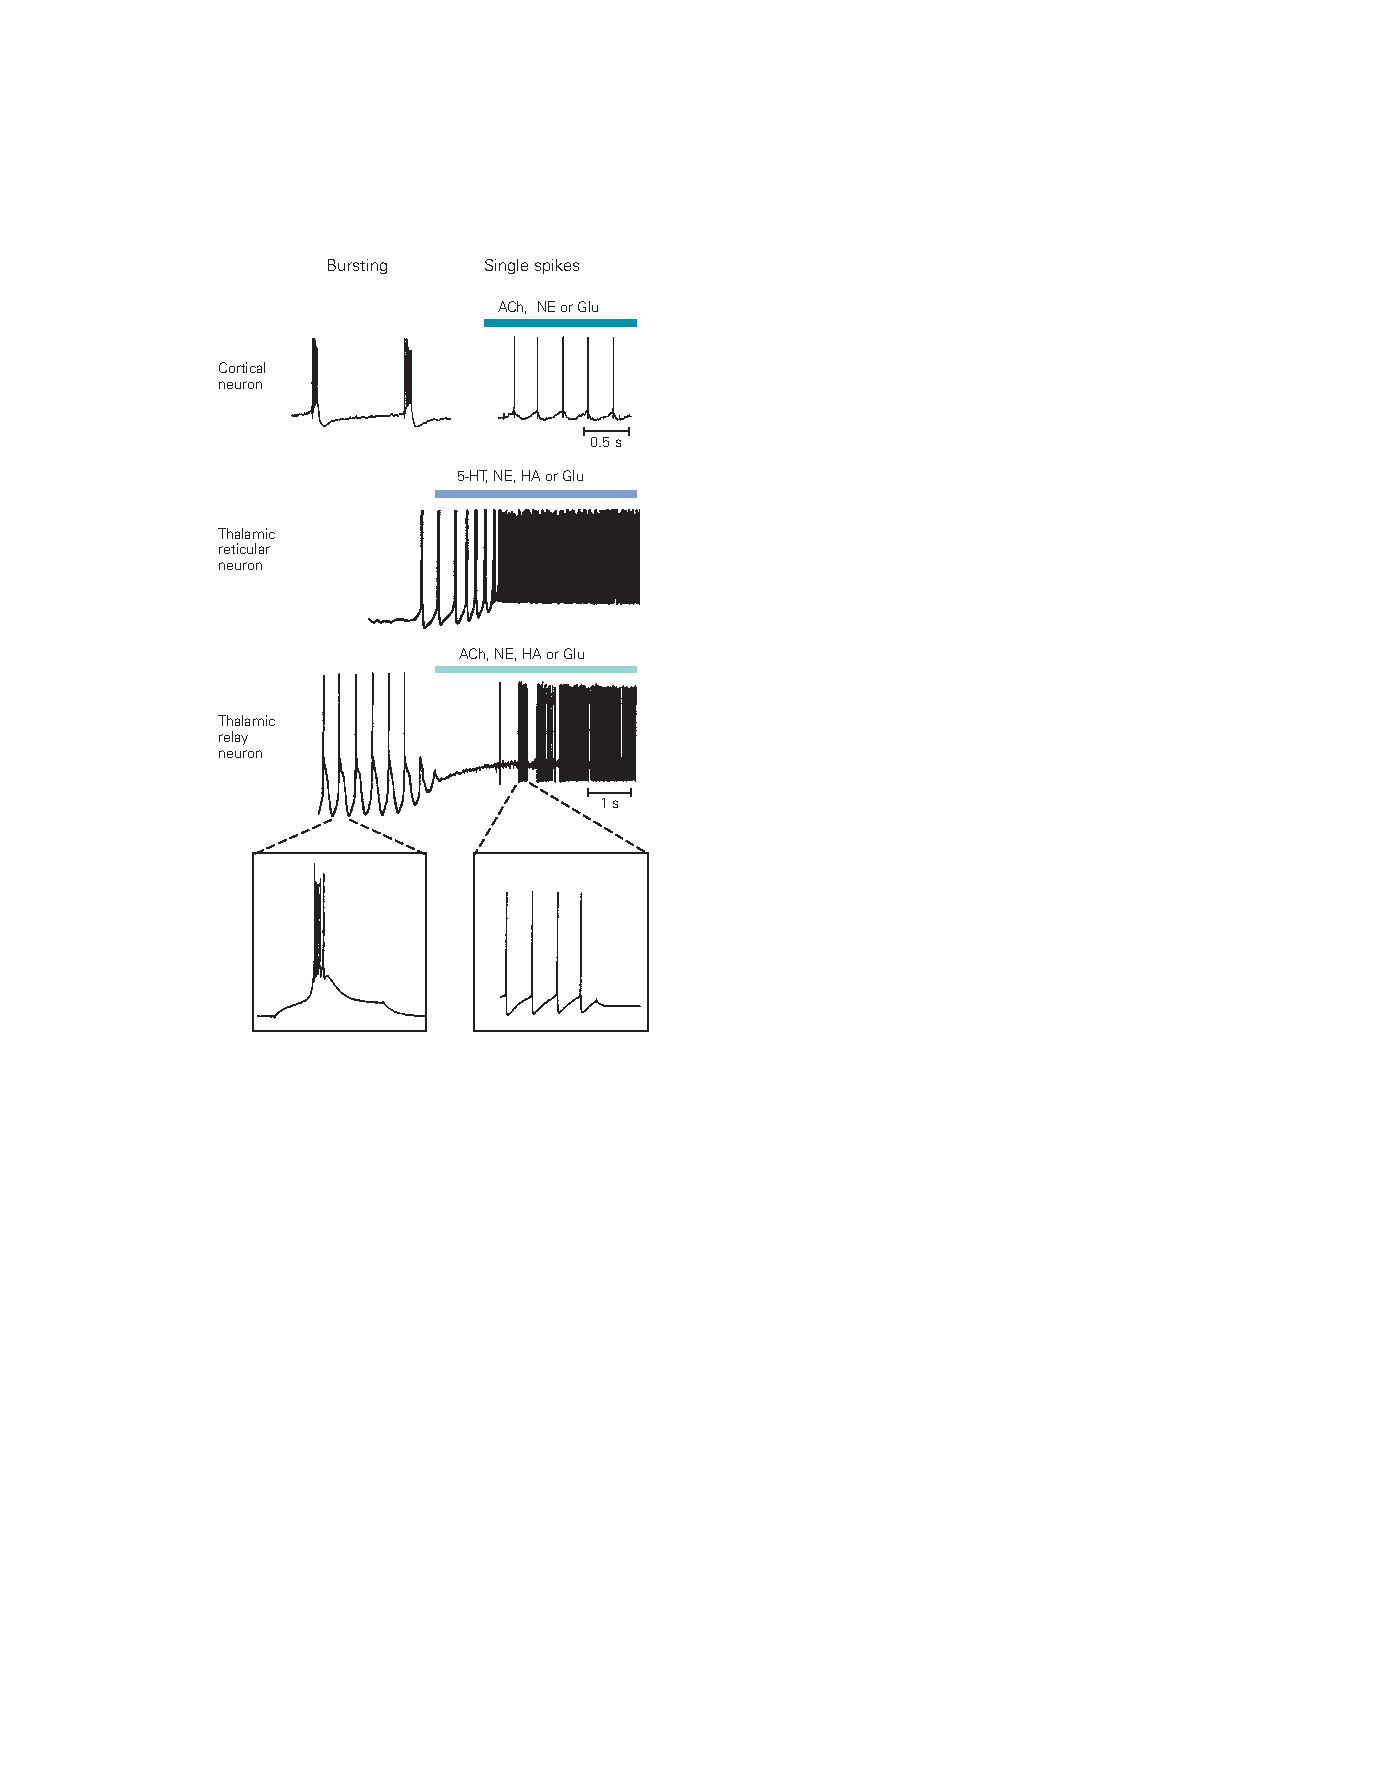
\includegraphics[width=0.5\linewidth]{chap40/fig_40_16}
	\caption{单胺能和胆碱能系统调节丘脑和皮层神经元的活动以维持觉醒。
		皮层和丘脑神经元的放电模式在乙酰胆碱或单胺的作用下从突发模式转变为单峰模式。
		录音来自脑切片中的神经元。
		丘脑和皮层神经元在有节奏地爆发时传递信息的能力有限。
		然而,当处于单尖峰模式时,它们的发射活动反映了它们接收到的输入。
		因此,单胺能和胆碱能唤醒系统保持皮层信息处理所需的通信线路畅通。
		(经许可转载自 Steriade、McCormick 和 Sejnowski 1993。版权所有 © 1993 AAAS。)}
	\label{fig:40_16}
\end{figure}


许多靶向单胺能和胆碱能系统的药物会影响觉醒。
例如,抗组胺药会导致困倦,血清素再摄取阻滞剂会减少快速眼动睡眠时间,而尼古丁是一种强大的兴奋剂。
此外,安非他明、可卡因和其他阻断多巴胺再摄取的药物会引起唤醒;
缺乏多巴胺转运蛋白的小鼠对此类药物不敏感。


帕金森病患者的黑质多巴胺能神经元丢失,蓝斑中的去甲肾上腺素能神经元也丢失,白天往往异常困倦。
一些用于治疗帕金森病的药物会激活剩余多巴胺能唤醒神经元突触前末端的 D2 多巴胺受体,从而导致突触前抑制,从而减少多巴胺释放。
因此,尽管这些药物可能会改善运动障碍(通过它们对纹状体神经元上突触后 D2 受体的影响),但对觉醒系统中剩余的多巴胺能细胞的抑制作用可能会加剧白天的嗜睡。



\section{要点}

1. 脑干和颅神经的计划在发育早期就展开了,因为神经元聚集成簇,及时形成它们的功能组织。
基于脊髓的基本结构,与面部、头部、颈部和内脏相关的运动和感觉神经元形成具有特定功能和神经支配区域的离散核。


2. 围绕这些脑神经核的网状结构中的神经元发育成神经元集合,这些神经元可以产生自主神经和运动反应的模式,这些反应有助于简单、刻板、协调的功能,从面部表情到进食和呼吸。
这些行为模式非常复杂和灵活,可以代表新生儿的整个行为库。


3. 随着前脑的发育和对这些脑干模式发生器的控制,各种更复杂的反应和最终的行为意志控制不断演变。


4. 然而,即使是熟练的演员也发现很难产生与特定情绪相关的面部表情,除非他在内部重建情绪状态,从而触发与这些感觉状态相关的预先模式化的面部表情。
因此,一些最复杂的人类情绪和行为是通过脑干中运动和自主反应的刻板模式无意识地表现出来的。


5. 脑干还包含一系列具有远程和弥散投射的细胞群。
他们的目标范围从大脑皮层的认知和行为系统,到下丘脑和脑干自主控制区,再到脊髓中的感觉和运动控制系统。
许多参与这些调节系统的神经元使用单胺作为神经调节剂,这些调节系统为更具体的感觉、运动、行为和自主神经输出设定了基调。


6. 由于这些调节途径的扩散和它们使用的受体的多样性,所有中枢神经系统活性药物中的很大一部分都作用于这些途径。
不幸的是,这些药物的许多脱靶效应是由于这些途径的扩散以及它们在多个位置使用相同的神经递质和受体。
中枢神经系统药理学未来面临的挑战将是开发对需要调节的目标功能更具选择性的药物。

